\documentclass[titlepage,a4paper]{article}


\usepackage[spanish,activeacute]{babel}
%\usepackage[margin = 1in]{geometry}
\usepackage{a4wide}
\usepackage{bookmark}
\usepackage{fancyhdr}
\usepackage{graphicx}

\pagestyle{fancy} % Encabezado y pie de página
\fancyhf{}
\fancyhead[L]{TP1  - Grupo: 38}
\fancyhead[R]{Teoría de organización de datos - FIUBA}
\renewcommand{\headrulewidth}{0.4pt}
\fancyfoot[C]{\thepage}
\renewcommand{\footrulewidth}{0.4pt}





\begin{document}

	\begin{titlepage}
		\hfill
\includegraphics[width=6cm]{logofiuba.jpg}
		\center
		\vfill
		\vfill
		\begin{center}
			\begin{Huge}\textbf{Trabajo Práctico Nº 1}\end{Huge}\\
			\vfill
			\begin{huge}Análisis Exploratorio\end{huge}\\
			\vfill
			\begin{Large} Teoría de Organización de Datos\end{Large}\\

			\textbf{Nombre grupo:} "The data inception" \\
			\textbf{Nº grupo: 38}\\
				Todo el trabajo realizado puede encontrarse en el siguiente repositorio de github:\textit{ https://github.com/sebalogue/tp1-datos.git. }
	
			\vfill
			\begin{tabular}{|c|c|c|}
				\hline
				participantes & nº padrón & mail \\ \hline
				LOIS,Lucas Edgardo & 98923 & lucaslois95@gmail.com \\ \hline		
				LOGUERCIO, Sebastian Ismael &100517 & seba21log@gmail.com \\ \hline
				MARIANI, Santiago Tomás &100516 &  santiagomariani2@gmail.com \\ \hline
				MARIJUAN, Magalí & 100070 & maguimar001@gmail.com\\ \hline
				
			\end{tabular}
			\vfill
			\vfill
			\vfill
			\vfill
			\vfill
			\vfill
		\end{center}
	
	\end{titlepage}

	\tableofcontents
	\newpage
	
	\section{Introducción}
	Este trabajo práctico consite en realizar un análisis sobre un conjunto de eventos de Web Analytics de usuarios que visitaron www.trocafone.com, su plataforma de ecommerce en Brasil. Trocafone es un side to side Marketplace para la compra y venta de dispositivos electrónicos que se encuentra actualmente operando en Brasil y Argentina.
	
	Para realizar dicho trabajo utilizaremos el lenguaje de programación \textit{Python}. Para el análisis de datos usaremos la librería \textit{Pandas} y para la realización de gráficos utilizaremos las librerías \textit{Matplotlib }y \textit{Seaborn}. Por otro lado, trabajaremos usando el sistema de control de versiones \textit{GIT}	
	
	El objetivo del trabajo práctico es analizar los distintos eventos e interacciones que pueden realizar los usuarios en la plataforma y a partir de estos establecer diversas conclusiones. Haremos énfasis en encontrar patrones de comportamiento y entender cuáles son las preferencias de los usuarios a la hora de comprar y vender productos teniendo en cuenta diversos parámetros, como la región en donde se originan, momento del día, semana del año, palabras clave, etc.
	
	Utilizaremos la siguiente abstracción para realizar el trabajo práctico: Se realizará una pregunta general, y a partir del uso de las herramientas mencionadas anteriormente se buscará dar una respuesta a partir del comportamiento de los datos.
	
	\section{Análisis Preliminar}
	En un primer análisis intentaremos entender cómo esta compuesto el dataset. Es decir, cuáles son los eventos que lo componenen, cómo interactúan en conjunto y cuáles son las características propias de cada evento. 
	\subsection{Eventos}
	El dataset contiene los siguiente eventos: 
	\begin{itemize}
	\item Viewed product: El usuario visita una página de producto.
	\item Brand listing: El usuario visita un listado específico de una marca viendo un conjunto de productos.
	\item Visited site: El usuario ingresa al sitio a una determinada url.
	\item Ad campaign hit:  El usuario ingresa al sitio mediante una campana de marketing online.
	\item Generic listing:  El usuario visita la homepage.
	\item Serched products:  El usuario realiza una búsqueda de productos en la interfaz de búsqueda del site.
	\item Search engine hit: El usuario ingresa al sitio mediante un motor de búsqueda web.
	\item Checkout: El usuario ingresa al checkout de compra de un producto.
	\item Staticpage: El usuario visita una página.
	\item Conversion: El usuario realiza una conversión, comprando un producto.
	\item Lead: El usuario se registra para recibir una notificación de disponibilidad de stock, para un producto que no se encontraba disponible en ese momento.
	\newpage
	La cantidad total de ocurrencias es:	1011288. Las cuales están distribuidas de la siguiente manera. 
	\end{itemize}
	\begin{center}
	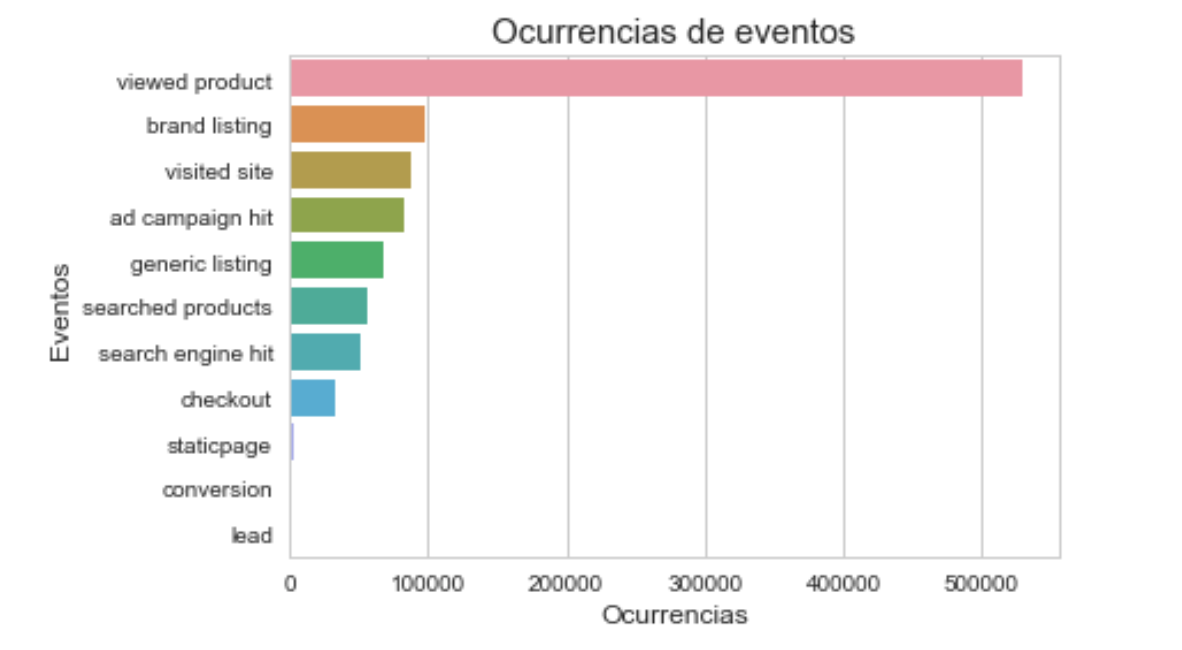
\includegraphics[width=15cm]{ocurrencia_eventos.jpg}\\
	\textbf{Figura 1:}  \textit{Cantidad de apariciones de cada evento. }
	\end{center}
	Es importante mencionar que no todos los campos del dataset participan en todos los eventos. Cada evento utiliza una determinada cantidad de columnas del dataset. Por lo tanto, mediante un análisis de elementos nulos llegamos a las siguiente conclusiones:
	\begin{itemize}
		\item Todos los eventos tienen timestamps qué indican exactamente en qué momento se realizo dicho evento. Además de poseer información sobre quien lo realizó. 
		\item Para el evento \textbf{viewed product} sus campos obligatorios son: timestamp , sku , model, condition, storage, color.
		\item Para el evento \textbf{brand listing} su campo obligatorio es: skus. 
		\item Para el evento \textbf{visited site} sus campos obligatorios son: channel, new vs returning, city, region, country, device tipe , screen resolution, operating system version y browser version.
		\item Para el evento \textbf{ad campaing hit} sus campos obligatorios son: url  y campaing source.
		\item Para el evento \textbf{generic listing} su campo obligatorios es: skus.
		\item Para el evento  \textbf{serched product } sus campos obligatorios son: skus y search term.
		\item Para el evento \textbf{serched engine} su campo obligatorio es: search engine
		\item Para el evento \textbf{checked out}  sus campos obligatorios son: sku, color, storage, model y condition 
		\item Para el evento \textbf{static page}  sus campo obligatorio es: satatic page
		\item Para le evento \textbf{conversion} sus campos obligatorios son:  sku, model, color , condition y storage
		\item Para el evento \textbf{lead} su campo obligatorio es: model
	\end{itemize}	
	Analizaremos a partir de los timestamps cuál es el momento del día en que se registra mayor actividad.
	\begin{center}
	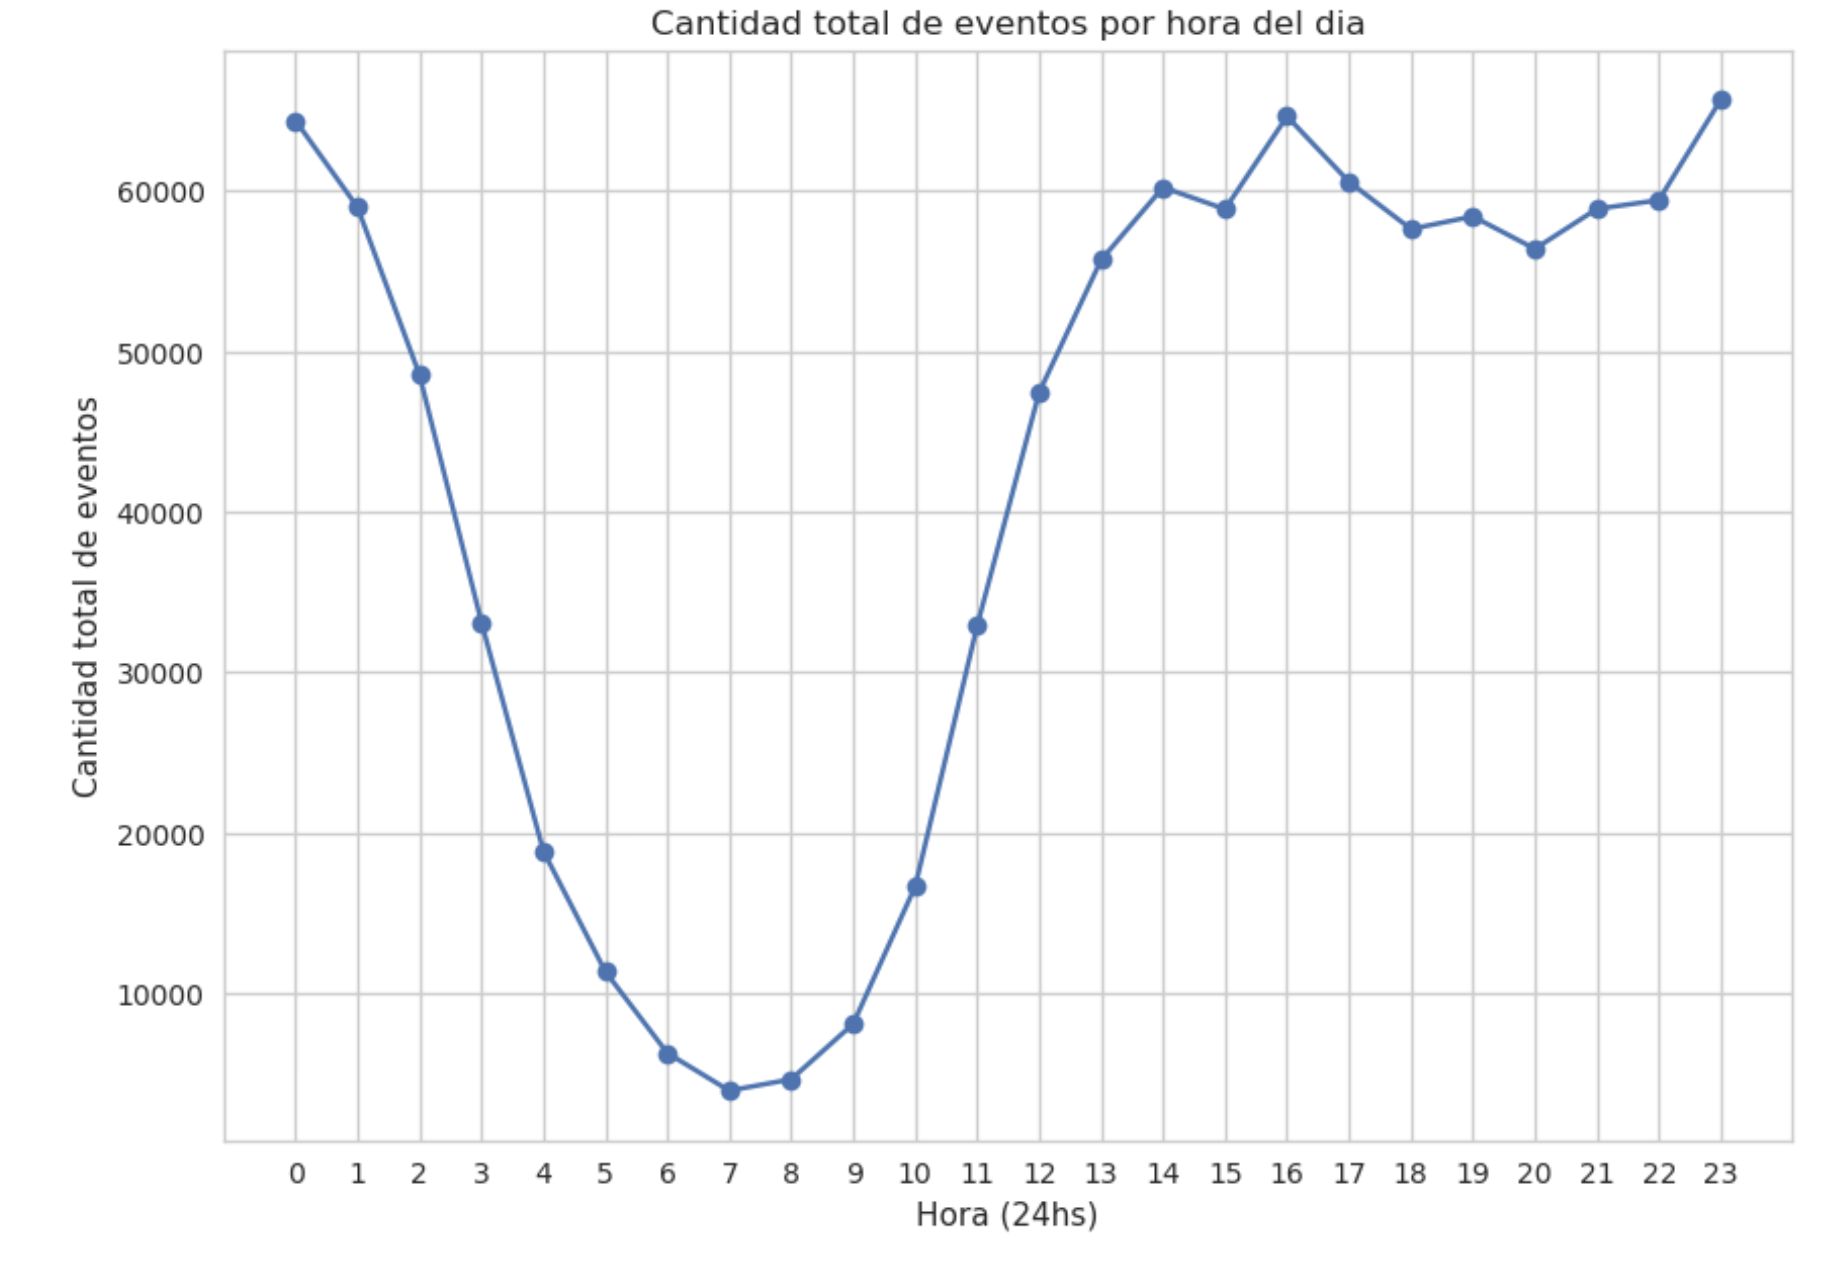
\includegraphics[width=13cm]{cantidadDeEventosPorHoraDelDia.jpg}\\
	\textbf{Figura 2:}  \textit{Distribución de los eventos a lo largo del día.}
	\end{center}
	Podemos observar que la mayoría de los eventos se efectúan entre las 14 hs y 2 hs. \\
	\subsection{Viewed product}
	\subsubsection{Análisis individual de las características}
	La primera columna que decicimos analizar de éste evento es model. Podemos observar cuáles son los modelos más visitados en el sitio:
	\begin{center}
	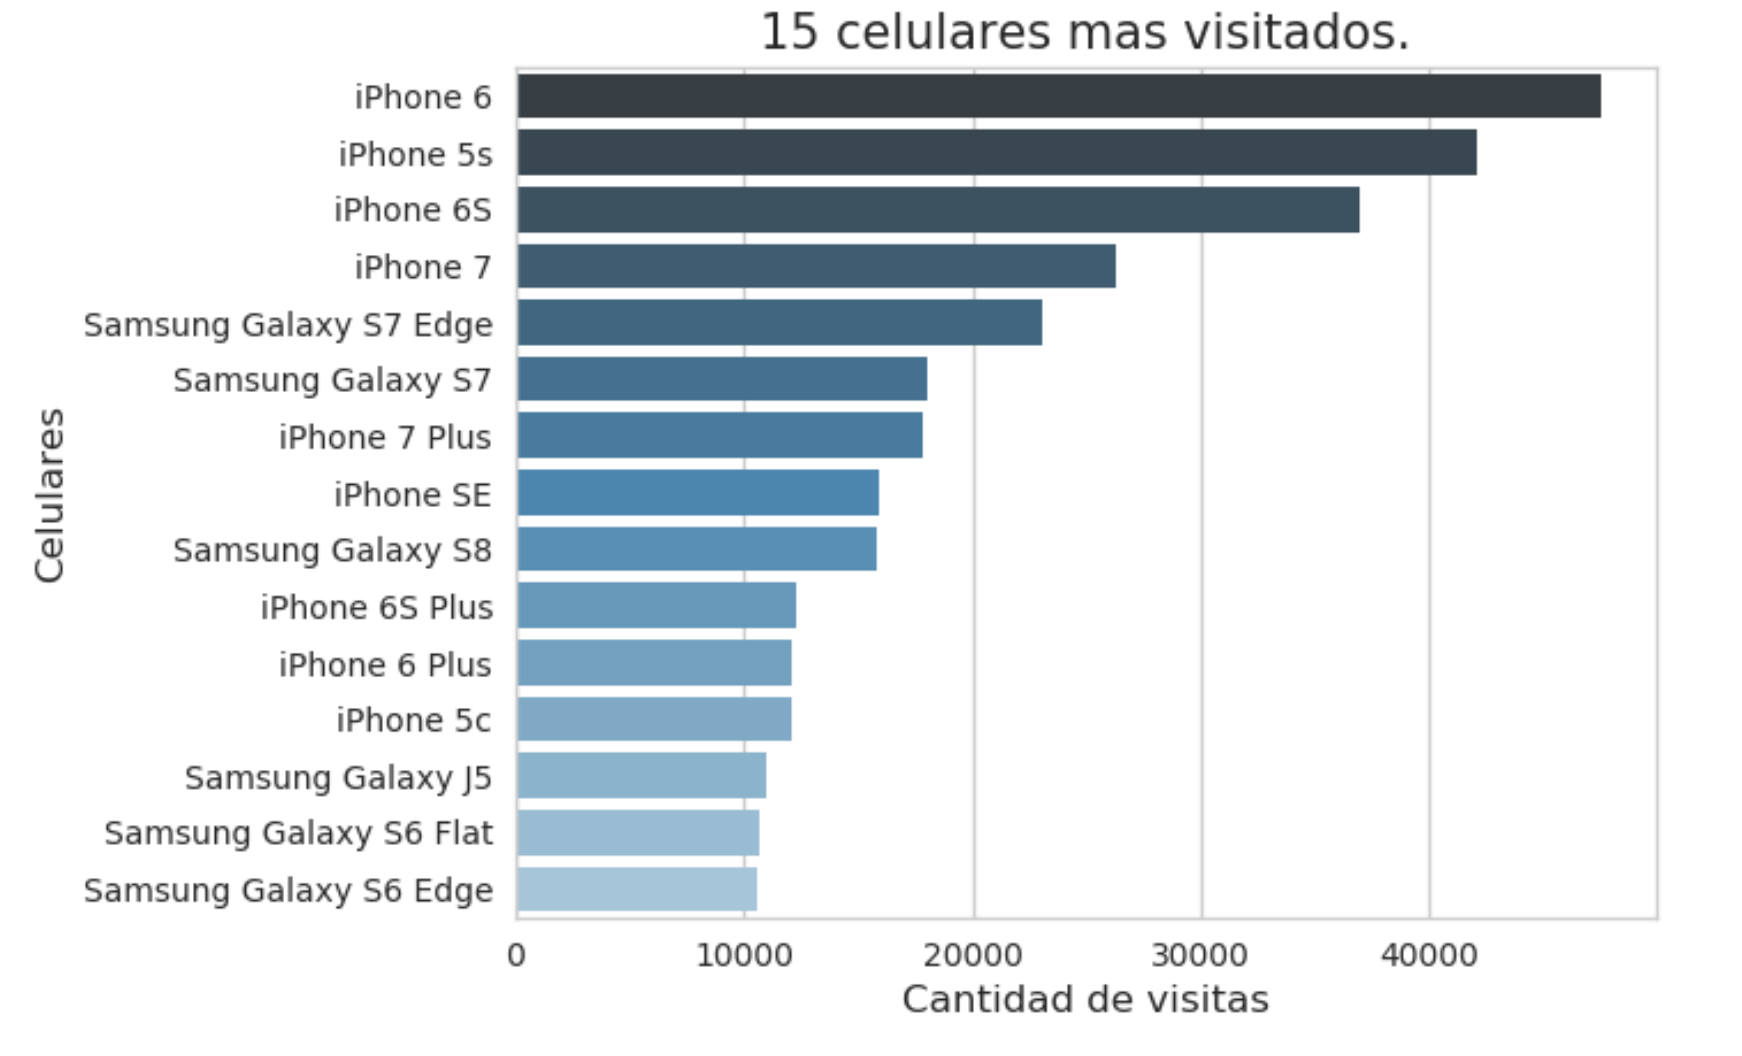
\includegraphics[width=15cm]{15celularesMasVisitados.jpg}\\
	\textbf{Figura 3:}  \textit{Cantidad de visitas por celular.}
	\end{center}
	 Sobre las características de esos modelos primero analizamos el color de los productos vistos y concluímos que el 50\% de las visitas se concentraron en los siguientes colores:
	\begin{itemize}
	\item el 23\% de las visitas es hacia productos negros.
	\item el 20\% de las visitas es hacia productos dorados.
	\item el 11\% de de las visitas es hacia productos gris espacial.
    \item el 10\% de de las visitas es hacia productos blancos.
     \item el 9\% de de las visitas es hacia productos plateados.
     \item el 6\% de de las visitas es hacia productos rosas.
	\end{itemize}	   
	Despreciamos el resto de los colores ya que el porcentaje de visitas es poco significativo. \\  \\
	Luego analizamos las visitas hacia el almacenamiento de los productos y concluímos que:
	\begin{itemize}
	\item El 33\% de las visitas es hacia productos con almacenamiento de 16 GB.
    \item El 32\% de las visitas es hacia productos con almacenamiento de 32 GB.
    \item El 17\% de las visitas es hacia productos con almacenamiento de 64 GB.
    \item El 6\% de las visitas es hacia productos con almacenamiento de 8 GB.
	\end{itemize}
	Por último analizamos las condiciones que más visita la gente y concluímos que:
	\begin{itemize}
    \item El 42\% de las visitas es hacia productos que son de calidad buena.
    \item El 27\% de las visitas es hacia productos que son de calidad excelente .
    \item El 27\% de las visitas es hacia productos que son de calidad muy buena.
        \item El 2\% de las visitas es hacia  productos que tienen identificador de huella digital. 
        	\item El 0,02\%  de las visitas es hacia  productos nuevos.    
	\end{itemize}
	\subsubsection{Análisis temporal}
	Estudiaremos en primer lugar cuáles son los días en los que se registraron la mayor cantidad de visitas.
	
		\begin{center}
	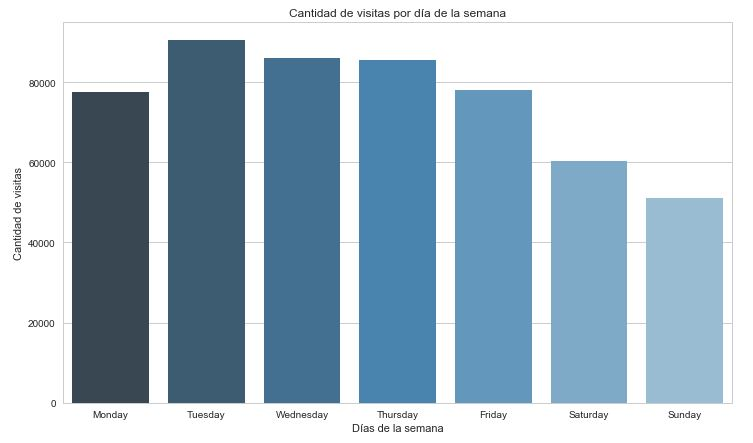
\includegraphics[width=15cm]{cantidadDeVisitasPorDiaDeLaSemana.jpg}\\
	\textbf{Figura 4:}  \textit{Cantidad de visitas según día del año.  }
	\end{center}
	
	Luego, realizaremos un análisis sobre cómo es el progreso de las visitas a lo largo del semestre.
	\begin{center}
	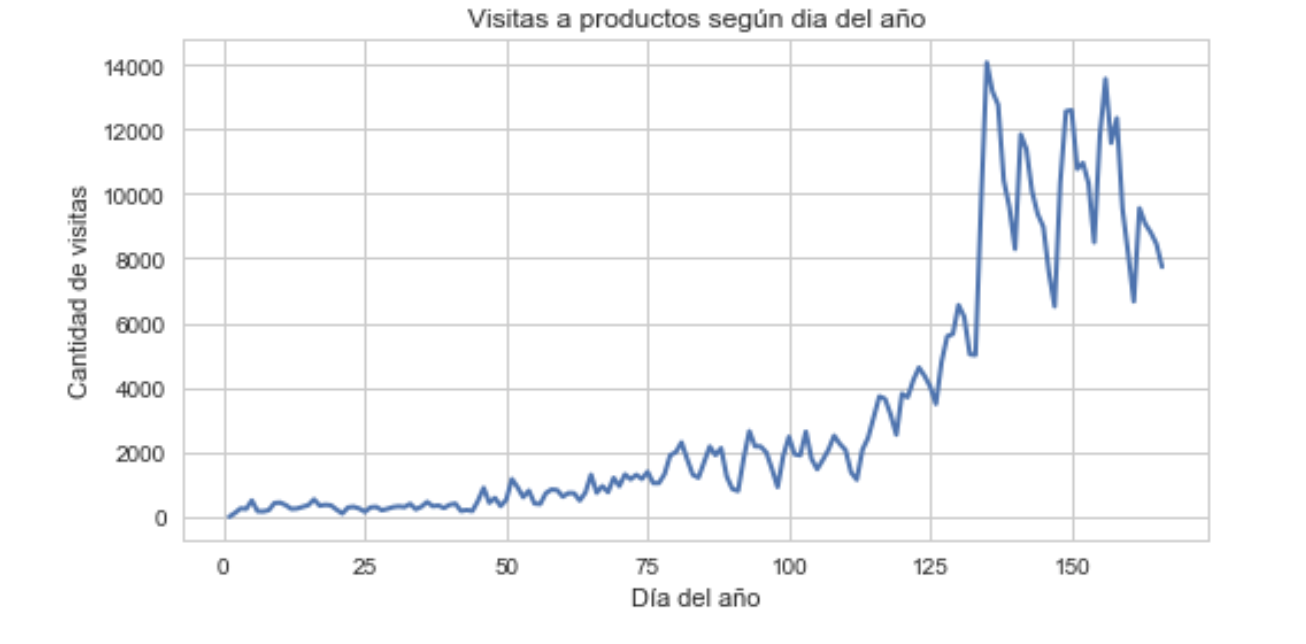
\includegraphics[width=15cm]{VisitasAProductosSegunDiaAnio.jpg}\\
	\textbf{Figura 4:}  \textit{Cantidad de visitas según día del año.  }
	\end{center}

	\begin{center}
	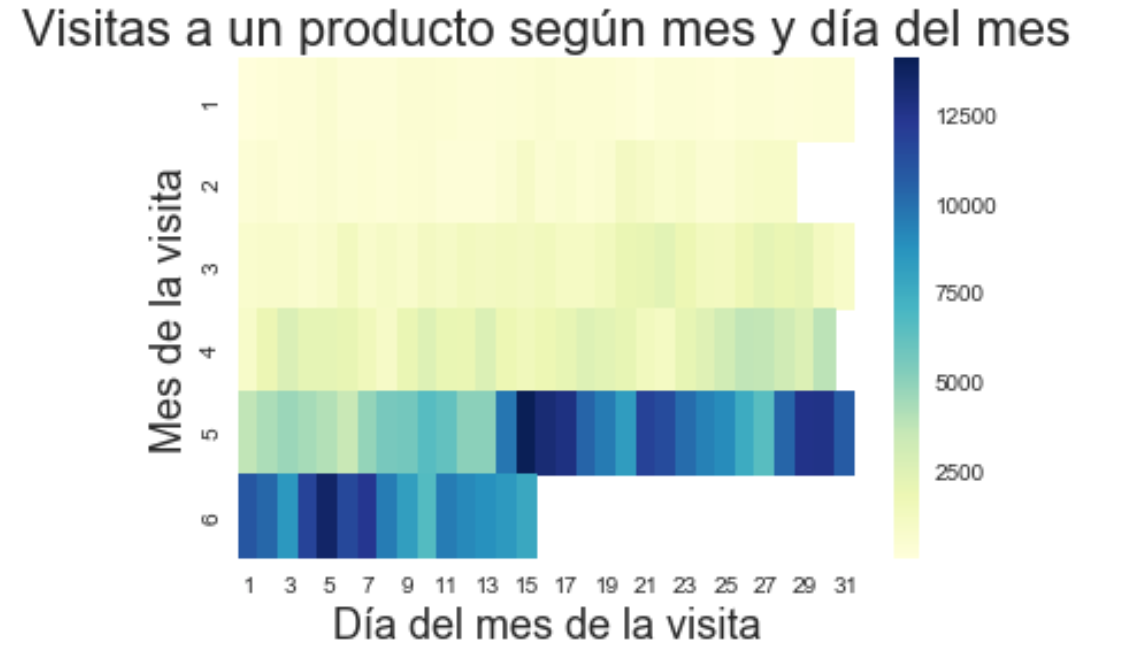
\includegraphics[width=15cm]{visitasSegunmesDiaMes.jpg}\\
	\textbf{Figura 5:}  \textit{Cantidad de visitas por cada día de cada mes. }\\
	Podemos notar que hay un fuerte incremento de actvidad a partir del 15 de mayo. 
	
	\end{center}
	\begin{center}
	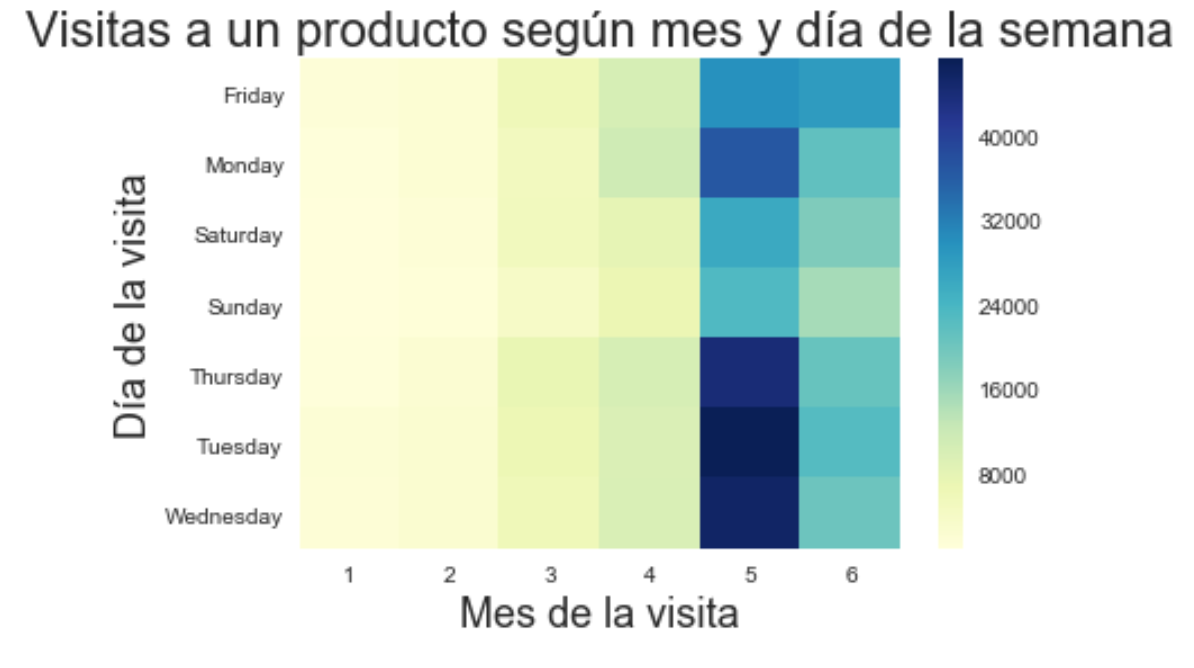
\includegraphics[width=15cm]{visitasSegunMesYDiaDeSemana.jpg}\\
	\textbf{Figura 6:}  \textit{Cantidad de visitas por cada día de semana de cada mes.   }
	\end{center}
	Nuevamente hay un fuerte incremento a partir del mes de mayo. Sin embargo, no parece haber una predominancia cuando hablamos de los días de la semana. Lo que podemos concluir es que los domingos hay menos actividad. 
	
	\textbf{Es importante destacar en el análisis temporal que el mes de  junio no está completo. Sólo tenemos datos de su primera quincena. }
	
	\subsubsection{Análisis cruzado}
	Por último relacionaremos todas las careacterísticas analizadas anteriormente entre sí. Primero entrelazaremos la información entre los cinco Iphones más vistos y su color (Analizaremos los iphones ya que su esquema de colores es uniforme). 

	\begin{center}
	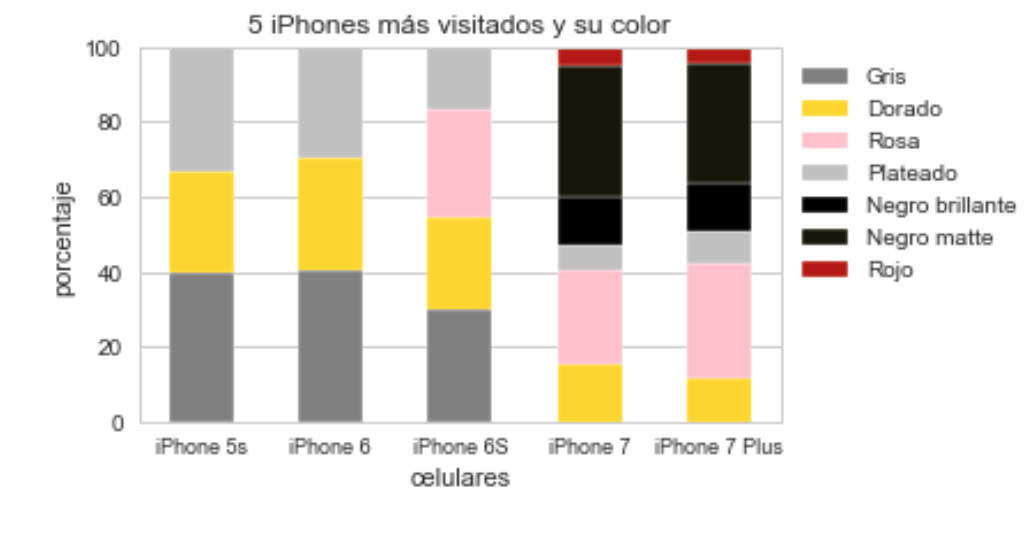
\includegraphics[width=15cm]{cincoModMasVisitadosColor.jpg}\\
	\textbf{Figura 7:}  \textit{Top 5 de celulares según su color. }
	\end{center}
	Por último, entrelazremos información entre los cinco modelos más visitos y su almacenamiento. 
	\begin{center}
	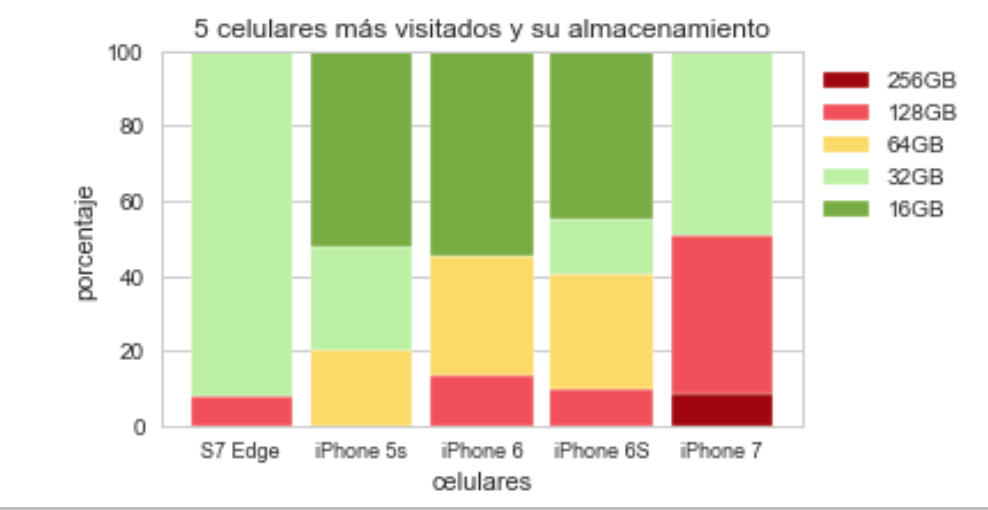
\includegraphics[width=15cm] {cincoModMasVisitadosAlmacenamiento.jpg}\\
	\textbf{Figura 8:}  \textit{Top 5 de celulares según su almacenamiento. }
	\end{center}
	Analizamos la cantidad de vistas de cada marca en cada semana del año.
	\begin{center}
	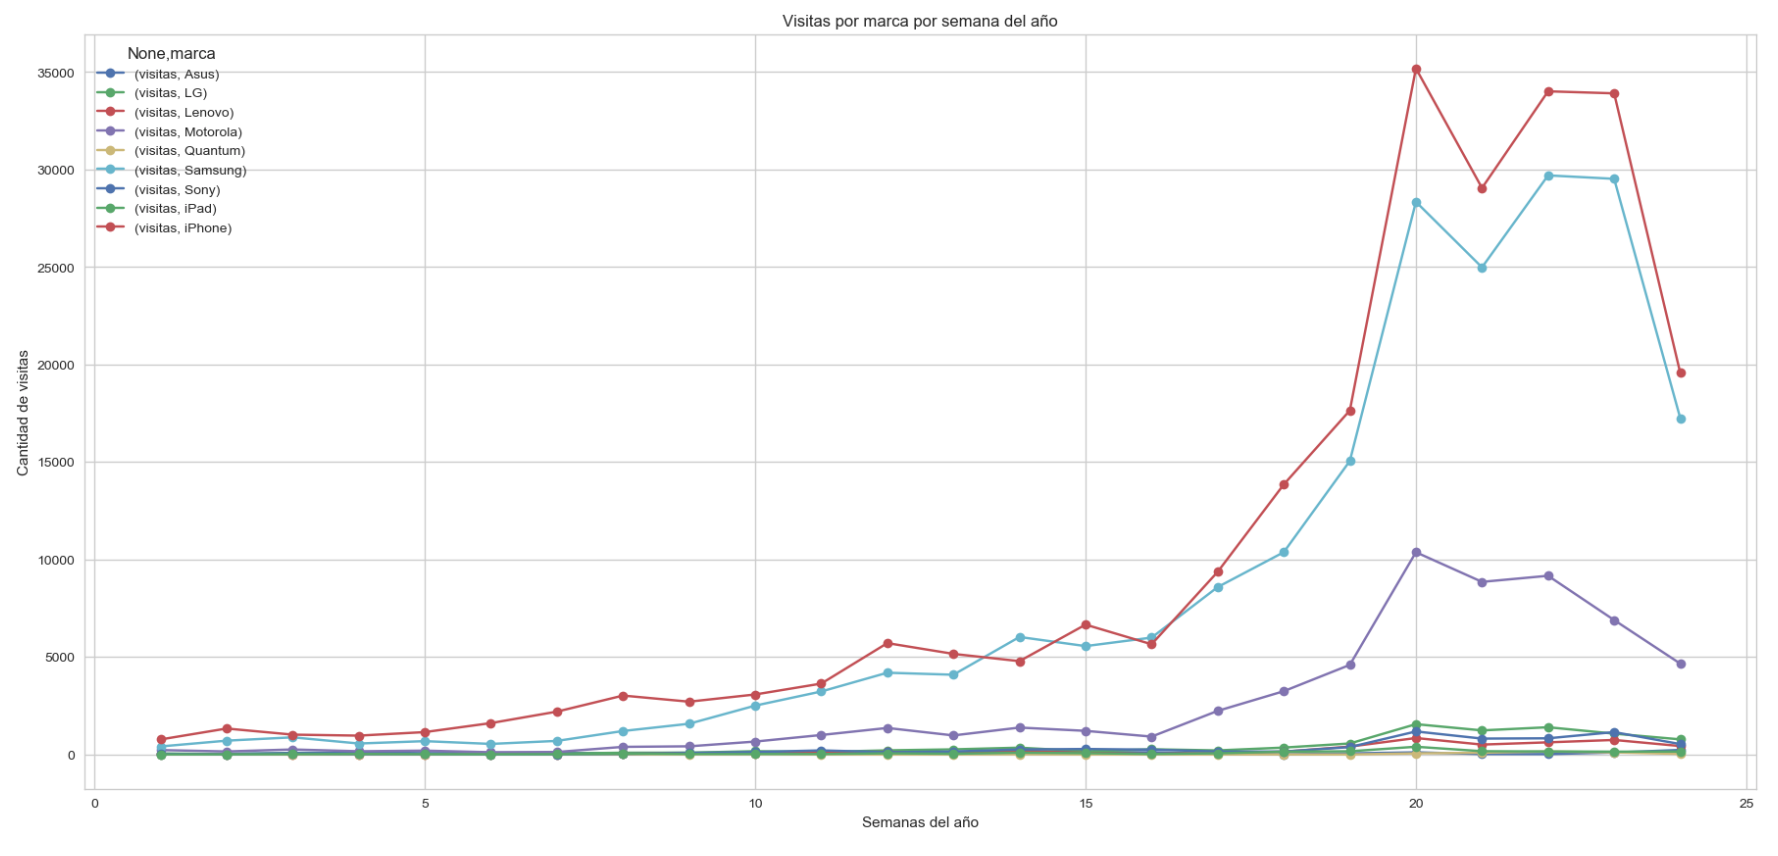
\includegraphics[width=15cm,height = 10cm] {visitasPorSemanaDelAnioPorMarca.jpg}\\
	\textbf{Figura 9:}  \textit{Progreso de visitas de cada marca por semana del año. }
	\end{center}	
	Concluímos que a partir de la semana 20 se produjo una explosión de visitas a los productos de marca  Apple y marca Samsung. 
	
	Por otra parte, analizaremos cuál es el progreso de compra de cada marca a lo largo del tiempo.	
	
		\begin{center}
	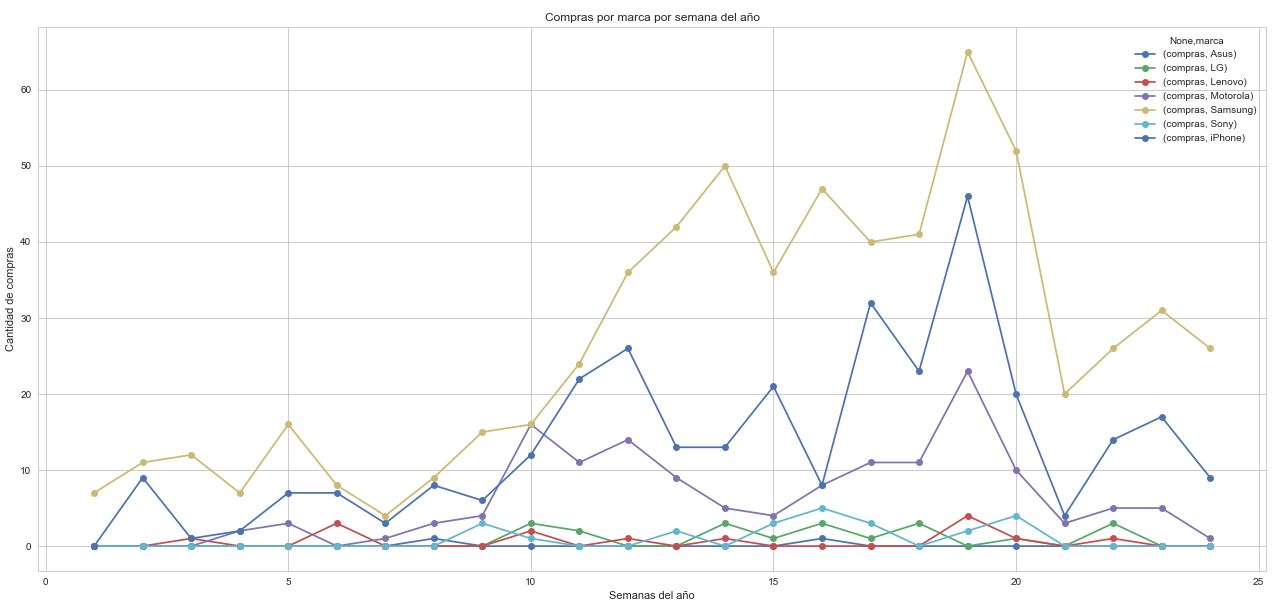
\includegraphics[width=15cm] {comprasPorMarcaPorSemanaDelAno.jpg}\\
	\textbf{Figura 8:}  \textit{Progreso de ventas de cada marca por semana del año. }
	\end{center}
	
	Podemos notar que si bien iPhone lidera las visitas del sitio a lo largo de las semanas, la mayor cantidad de compras las poseen los productos de Samsung.	
	
	\subsection{Ad campaign Hit}
	Indica cuando un usuario se conecta a partir de una campaña publicitaria.
	\subsubsection{Análisis individual de las caracterísiticas}
	Comenzamos analizando este evento fijandonos cuál es la fuente que produce la mayor cantidad de visitas.
	\begin{center}
	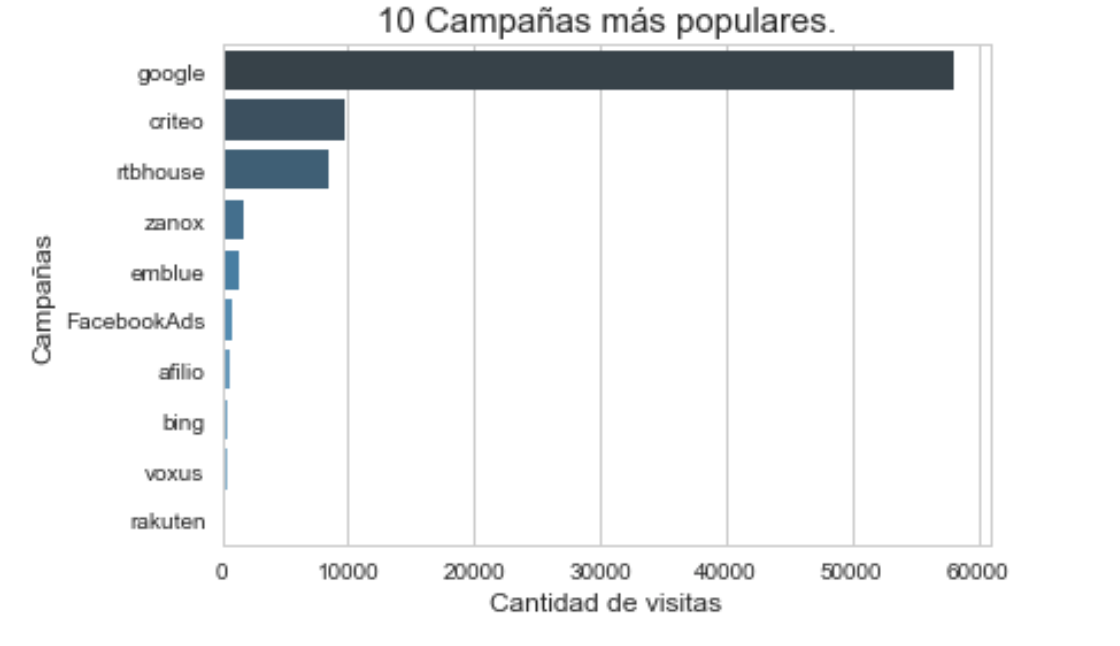
\includegraphics[width=13cm] {10campaniasmasPopulares.jpg}\\
	\textbf{Figura 10:}  \textit{Las fuentes de campañas publicitarias que generaron la mayor cantidad de visitas.  }
	\end{center}
	Ad campaign hit se divide en tres tipos de accesos: página principal, ventas y compras. Obtuvimos que: 
	\begin{itemize}
	\item El 65\% de los accesos es a compras.
	\item El 34\% de los accesos es a la página principal.
	\item El 0,26\% de los accesos es a ventas. 
	\end{itemize}
	El acceso según ventas puede clasificarse según la marca. Obtuvimos lo siguiente: 
	\begin{center}
	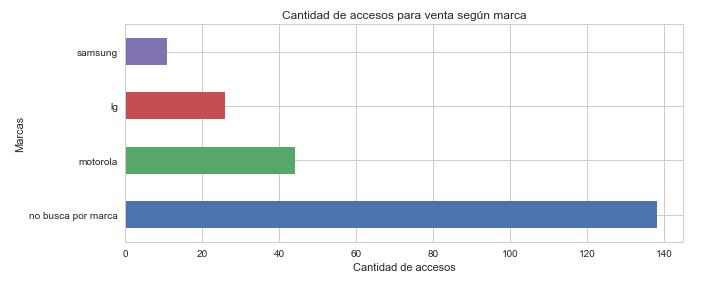
\includegraphics[width=12cm] {cantidadDeAccesosPorMarca.jpg}\\
	\textbf{Figura 11:}  \textit{Cantidad de accesos para venta según la marca.}
	\end{center}
	Este acceso tambien puede clasificarse según el modelo. Obtuvimos lo siguiente:
	\begin{center}
	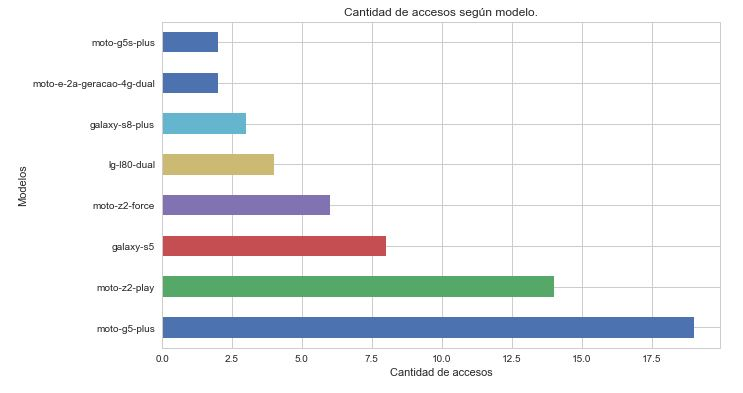
\includegraphics[width=12cm] {cantidadDeAccesosPorModelo.jpg}\\
	\textbf{Figura 12:}  \textit{Cantidad de accesos para venta según el modelo.}
	\end{center}
	El acceso según compras puede clasificarse según la marca. Obtuvimos lo siguiente:
	\begin{center}
	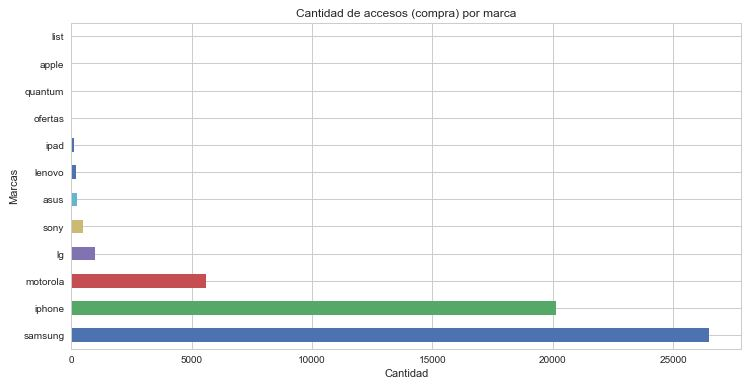
\includegraphics[width=15cm] {cantidadDeAccesosPorMarcaCompra.jpg}\\
	\textbf{Figura 13:}  \textit{Cantidad de accesos para compra según la marca}
	\end{center}
	El acceso de compras por oferta es poco significativo,por eso no lo excluímos del gráfico.\\
	Hacer un análisis de las compras según modelo es muy complicado y no creemos que valga la pena. Esto se debe a que un mismo modelo puede tener urls distintos. 
	\subsubsection{Análisis temporal}
	Analizamos las cinco campañas publicitarias más clickeadas a lo largo de los meses. Lo obtenido es: 
	\begin{center}
	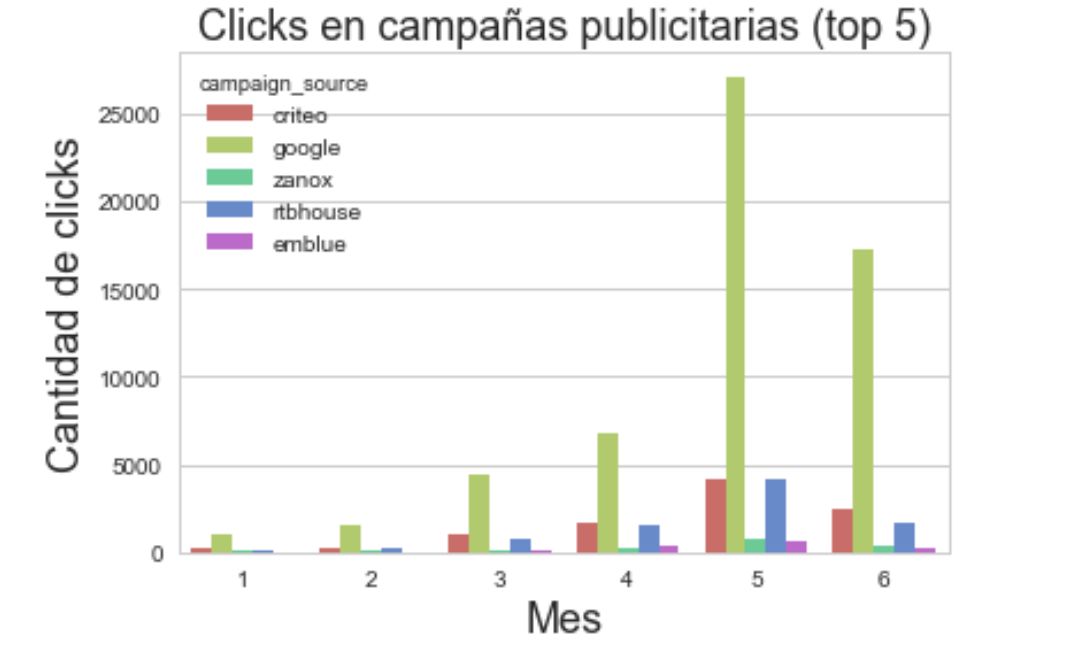
\includegraphics[width=15cm] {top5campaniasPublicitariasMasImportantesSegunMes.jpg}\\
	\textbf{Figura 14:}  \textit{Cantidad de clicks según campaña por mes.}
	\end{center}
	Analizamos así tambien el top5 de campañas publicitarias según la cantidad de clicks  en cada día del año. Obtuvimos lo siguiente:
	\begin{center}
	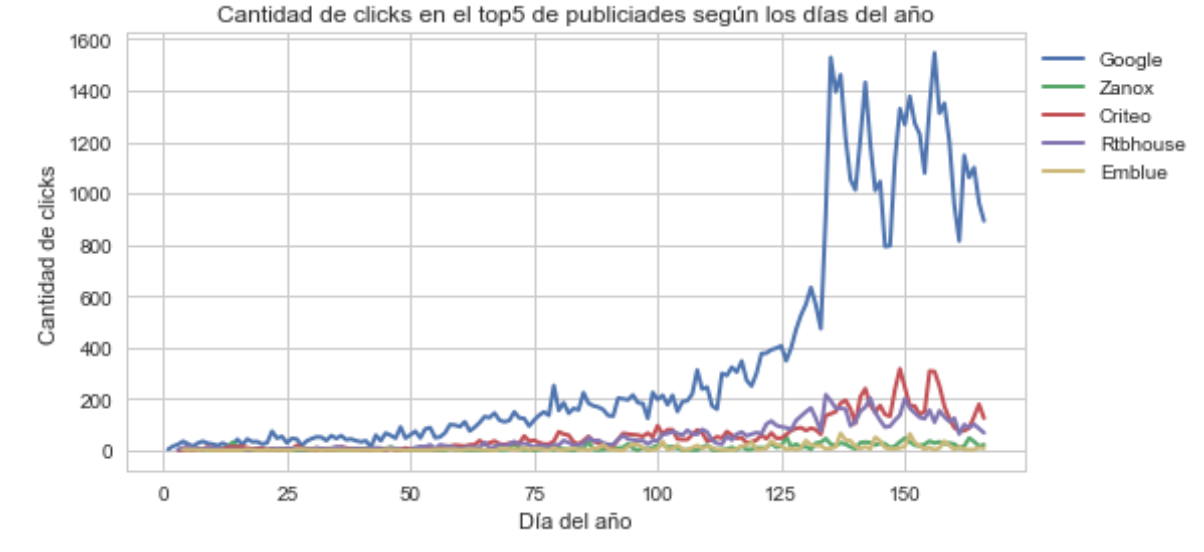
\includegraphics[width=15cm, height = 10cm] {cantidadDeClicksSegunDiaDelAnio.jpg}\\
	\textbf{Figura 15:}  \textit{Cantidad de clicks según campaña por día del año.  }
	\end{center}
	\subsection{Checkout}
	\subsubsection{Análisis individual de las caracterísiticas}
	Empezamos analizando los 10 modelos que más llegaron al checkout. Ellos son:
	\begin{itemize}
	\item iPhone 6 con el 10\% de los checkouts.
	\item iPhone 5s con el 8\% de los checkouts.
	\item iPhone 6S  con el 7\% de los checkouts.
	\item Samsung Galaxy J5 con el 6\% de los checkouts.
	\item Samsung Galaxy S7 con el 4\% de los checkouts.
	\item iPhone 7 con el 4\% de los checkouts.
	\item Samsung Galaxy S8 con el 3\% de los checkouts.
	\item iPhone 7 Plus con el 3\% de los checkouts.
	\item Samsung Galaxy J7 Prime con el 3\% de los checkouts.
	\item Samsung Galaxy S6 Flatcon el 3\% de los checkouts.
	\end{itemize}
	Analizamos la cantidad de checkouts según el almacenamiento. Lo obtenido es:
	\begin{itemize}
	\item El 37\% de los checkouts fue de dispositivos de 16GB
	\item El 29\% de los checkouts fue de dispositivos de 32GB
	\item	El 16\% de los checkouts fue de dispositivos de 64GB
	\item	El 11\% de los checkouts fue de dispositivos de 8GB
	\item	El 5\% de los checkouts fue de dispositivos de 128GB
	\item	El 1\% de los checkouts fue de dispositivos de 4GB
	\item	El 1\% de los checkouts fue de dispositivos de 256GB
	\item	El 0,1\% de los checkouts fue de dispositivos de 512MB
	\end{itemize}
	Analizamos la cantidad de checkouts según el color. Lo obtenido es:
	\begin{center}
	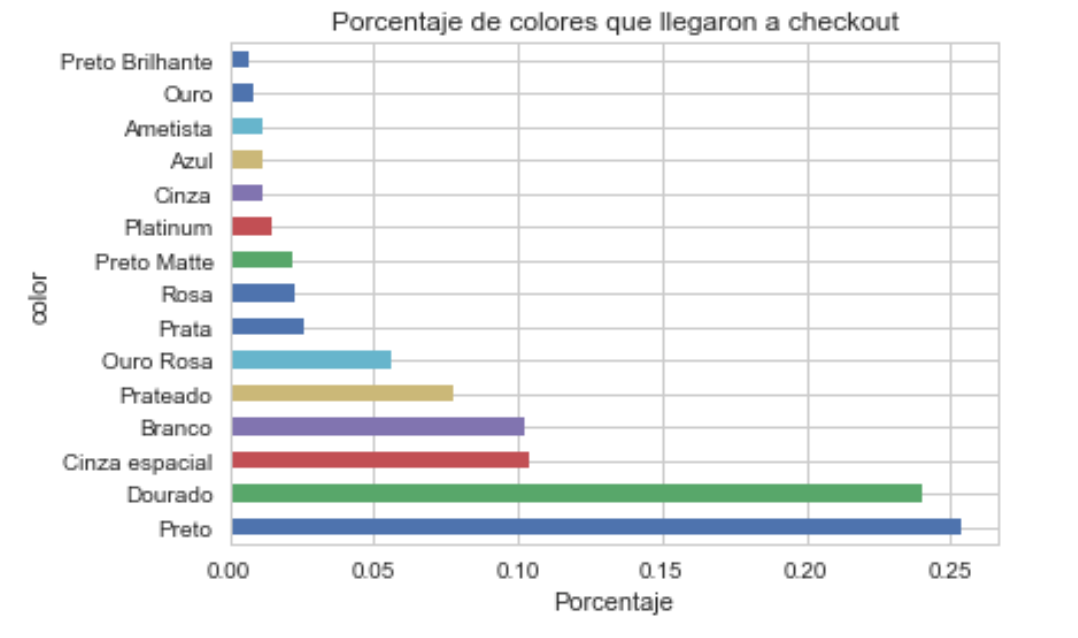
\includegraphics[width=15cm] {porcentajeDeColoresQueLlegaronACheck.jpg}\\
	\textbf{Figura 16:}  \textit{Porcentaje de colores que llegaron al checkout.}
	\end{center}
	Por último analizamos la condición de los productos que llegaron al checkout. Lo obtenido fue:
	\begin{itemize}
	\item El 45 \% de los productos son de condición buena. 
	\item El 27\% de los productos son de condición excelente.
	\item El 24\% de los productos son de condición muy buena. 
	\item El 3\% de los productos son de condición buena con touch id. 
	\item No es representativo la cantidad de productos nuevos. 
	\end{itemize}
	\subsubsection{Análisis temporal}
	Analizamos la cantidad de checkouts según los días del año. Obtuvimos lo siguiente:
	\begin{center}
	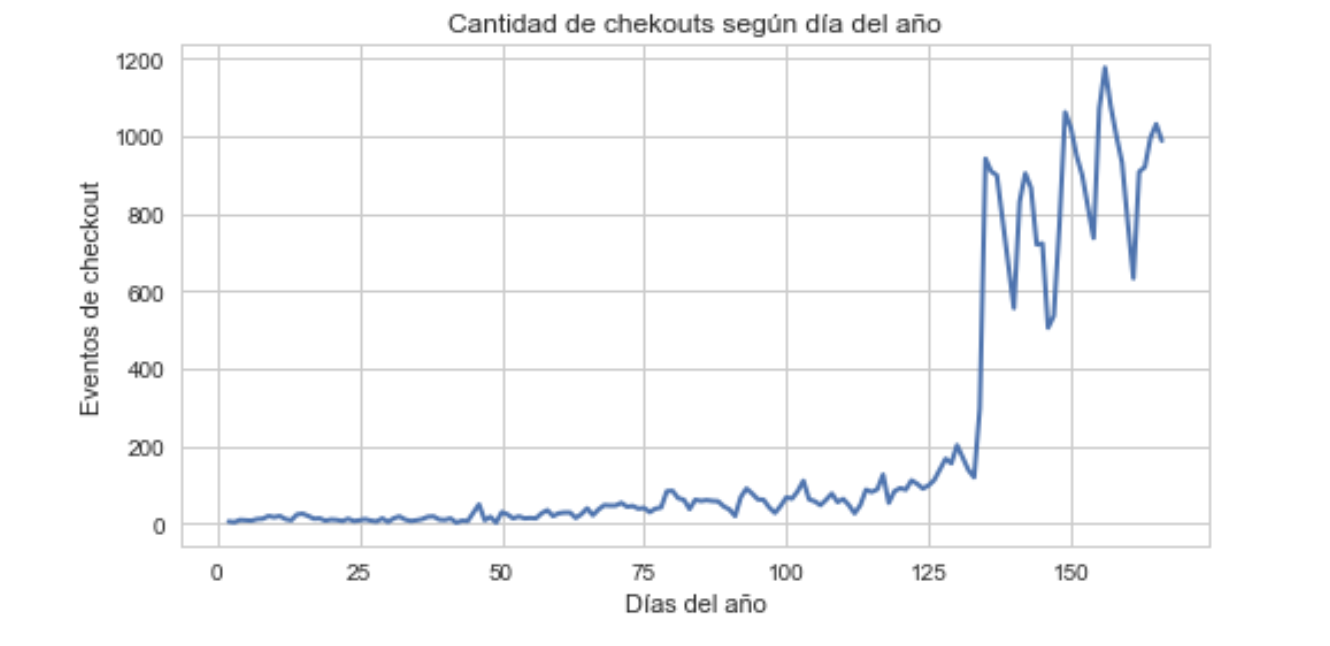
\includegraphics[width=13cm] {cantidadDeCheckoutsSegunDiaDelAnio.jpg}\\
	\textbf{Figura 17:}  \textit{Cantidad de checkouts según día del año.}
	\end{center}
	\subsection{Lead}
	\subsubsection{Análisis Individual de las caracterísiticas}
	Analizamos cuáles son los modelos no disponibles con más pedidos de notificación de stock. El resultado es:
	\begin{center}
	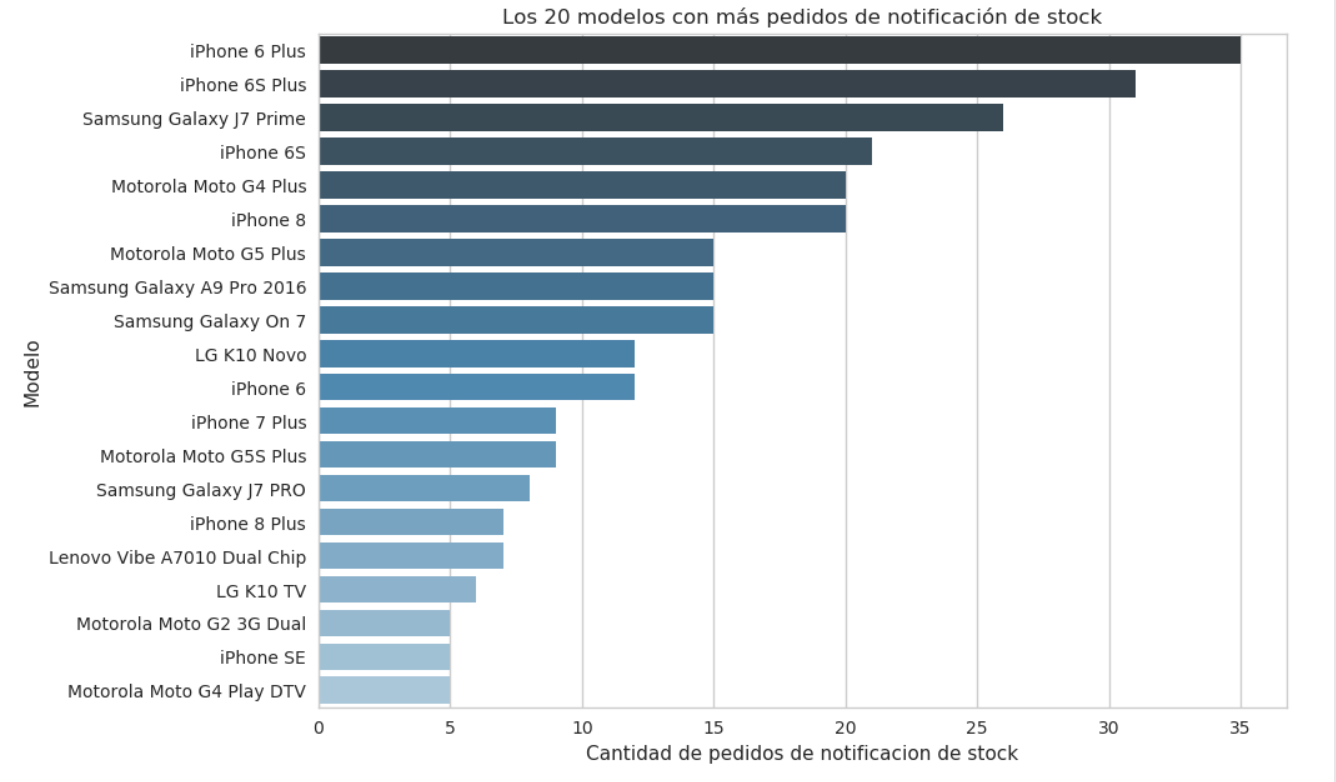
\includegraphics[width=15cm] {los20modelosConMasPedidosDeNotificacionDeStock.jpg}\\
	\textbf{Figura 18:}  \textit{Los 20 modelos con más pedidos de notificación de stock.}
	\end{center}

	Existe una relación del 8\% entre las veces que una persona agrega un determinado producto a Lead y este es comprado por la misma persona (ya sea por causa del Lead o por causa externa, no podemos determinarlo).
	
	Sabemos que como mucho el 8\% de las personas que agregaron un celular al Lead terminaron comprando este producto luego de haber recibido la correspondiente notificación.
	
	A pesar de que el porcentaje de conversiones en base al lead es bajo, es un factor importante a tener en cuenta ya que indica cuánto interés pueden tener los usuarios por comprar un producto cuando este no se encuentra en stock.
	
	\subsection{Brand listing} -> COMPLETAR
	\subsection{Visited site}
	Visitas recibidas en la página principal.
	\subsubsection{Análisis individual de las caracterísiticas}
	Comenzaremos por analizar cuáles son los países desde donde se efectúan las visitas, los más importantes son:
	\begin{itemize}
	\item Brasil con el  96\% de las visitas.
	\item Unknown con el  3\% de las visitas.
	\item United States con el 1\% de las visitas
	\end{itemize}
	Como Unknown representa un porcentaje tan pequeño decidimos omitirlo, de igual manera con el resto de los países. \\
	Como Brasil es el país predominante nos focalizaremos en analizar su comportamiento.
	
	\begin{center}
	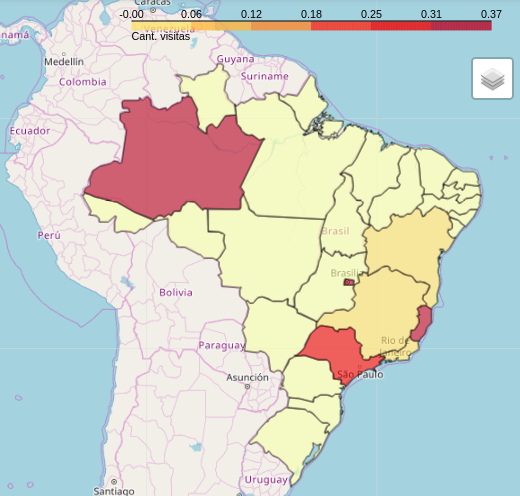
\includegraphics[width=15cm] {mapaEstadoBrasil.jpg}\\
	\textbf{Figura 19:}  \textit{Cantidad de vistas según estado de Brasil}
	\end{center}
	Podemos ver que la mayor cantidad de visitas se realizan desde Sao Paulo, 
Minas Gerais  y Rio de Janeiro .\\
	Analizaremos ahora las ciudades desde las que se produjeron la mayor cantidad de visitas.
	
	\begin{center}
	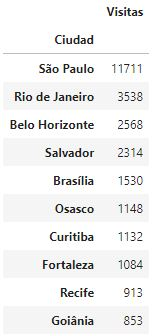
\includegraphics[width=4cm] {tablaVisitasPorCiudad.jpg}\\
	\end{center}		
	
	Como podemos observar, Sao Paulo es la ciudad que posee la mayor cantidad de visitas. Visualizaremos la relación entre las visitas de las ciudades a partir del siguiente gráfico.	
	
	\begin{center}
	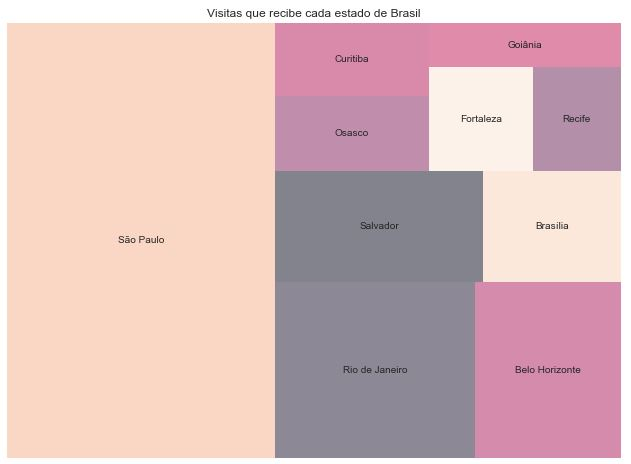
\includegraphics[width=15cm] {cantidadDeVisitasPorEstadoDeBrasil.jpg}\\
	\textbf{Figura 19:}  \textit{Cantidad de vistas según ciudad de Brasil}
	\end{center}	
	
	Procederemos por analizar los canales por los que se realizan las visitas. Los canales son: 
	\begin{itemize}
	\item Display: Interacciones con un medio de \textit{display} o \textit{cpm}. También incluye las interacciones de Google Ads con la red de distribución de anuncios configuradas como \textit{content}.
	\item Paid Search: Tráfico desde la red de motores de búsqueda, con un medio de \textit{cpc} o \textit{ppc}.
	\item Other: Sesiones etiquetadas con un medio de \textit{cpc}, \textit{ppc}, \textit{cpm}, \textit{cpv}, \textit{cpa}, \textit{cpp} o \textit{affiliate} (excluida la publicidad en buscadores).
	\item Organic Search: Tráfico de búsqueda gratuita en cualquier motor de búsqueda.
	\item Social Network: Tráfico de cualquiera de las aproximadamente 400 redes sociales (que no están etiquetadas como anuncios).
	\item Referral: Tráfico de sitios web que no son redes sociales.
	\item Email: Sesiones que están etiquetadas con el medio de \textit{email}.
	\item Direct: Sesiones en las que el usuario ha escrito la URL del sitio web en el navegador o ha llegado al sitio a través de un marcador.
	\end{itemize}
	Analizamos la cantidad de visitas por canal. El resultado es:
	\begin{center}
	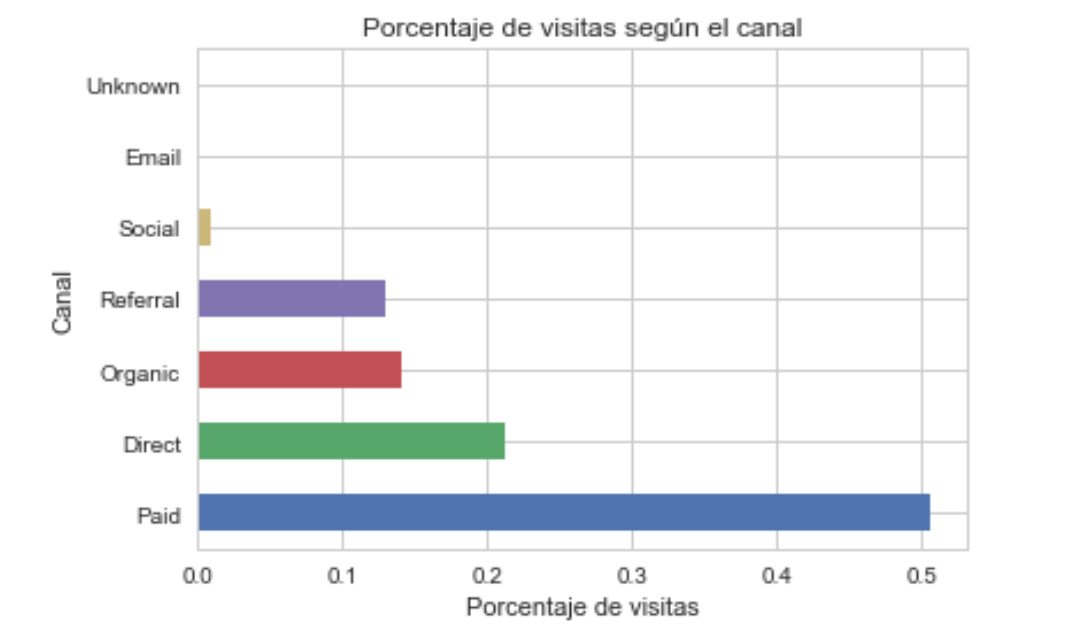
\includegraphics[width=15cm] {porcentajeDeVisitasPorCanal.jpg}\\
	\textbf{Figura 20:}  \textit{Porcentaje de visitas según el  canal}
	\end{center}
	Podemos ver que el canal predominante es paid seguido por direct. \\
	De este evento podemos obtener información acerca de cuales son los usuarios nuevos y cuales volvieron. La información obtenida es:
	
	\begin{center}
	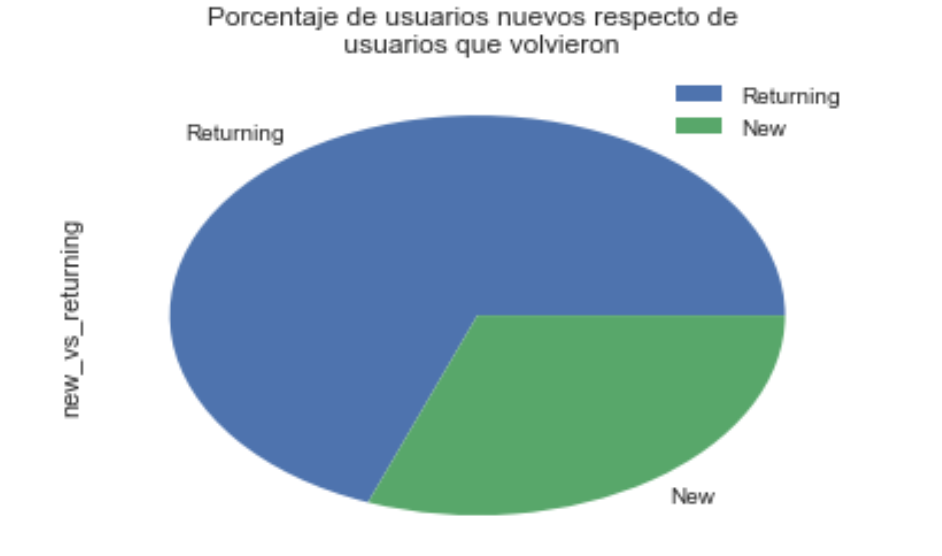
\includegraphics[width=10cm] {porcentajeUsuariosNuevosRespectoDeUsQueVolvieron.jpg}\\
	\textbf{Figura 21:}  \textit{Porcentaje de usuarios nuevos respecto de usuarios que volvieron. }
	\end{center}
	Podemos ver que el 69\% de la actividad registrada en el sitio proviene de retornos  y el  31\% de los usuarios nuevos. \\
	Analizando los dispositivos desde el cual acceden los usuarios obtuvimos que:
\begin{itemize}
\item El 50\% accede desde su teléfono
\item El 47\% accede desde su computadora
\item El 2\% no se sabe. 
\item El 1\% accede desde su tablet
\end{itemize}
	Procederemos por analizar las visitas desde los 15 sistemas operativos más populares. 
	\begin{center}
	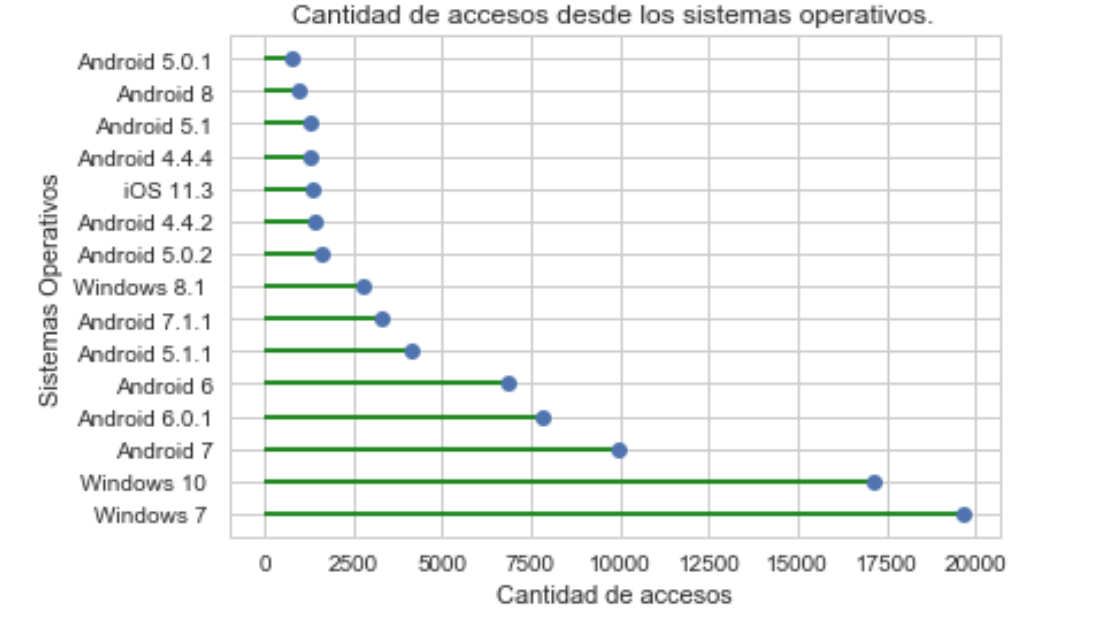
\includegraphics[width=15cm] {cantidadDeAccesosDesdeLosSistemasOperativos.jpg}\\
	\textbf{Figura 22:}  \textit{Cantidad de accesos por sistema operativo. Se muestran los 15 sistemas operativos más populares.}
	\end{center}
	
	Para analizar el retorno de los usuarios a la página, pudimos obtener la cantidad de usuarios que hubo por número de regresos al sitio. Es decir, mirando el gráfico: existieron \textit{y} cantidad de usuarios que regresaron \textit{x} cantidad de veces a la página.
	
	\begin{center}
   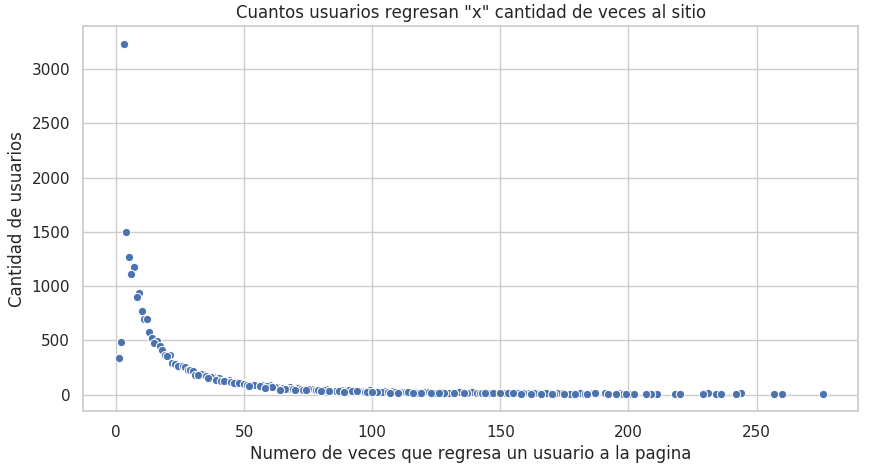
\includegraphics[width=14cm]{regresosPorUsuario.jpg}\\
	\textbf{Figura 23:}  \textit{Cantidad de usuarios por número de regresos a la página}
	\end{center}
	
   Se puede ver que gran parte de los usuarios estan más a la izquierda del gráfico. Es decir, el numero de regresos a la página es menor. La cantidad de usuarios disminuye a medida que se mira más adelante en el eje horizontal (a más cantidad de regresos al sitio).   
   
 Es interesante ver que existe un pico que se destaca en el numero 3 (usuarios que regresan 3 veces) y ver que hay mas usuarios que regresan entre 3 y 14 veces que los que regresan 1 o 2 veces. Aquí se muestra un gráfico de barras mostrando lo último descrito.	
 
	 \begin{center}
   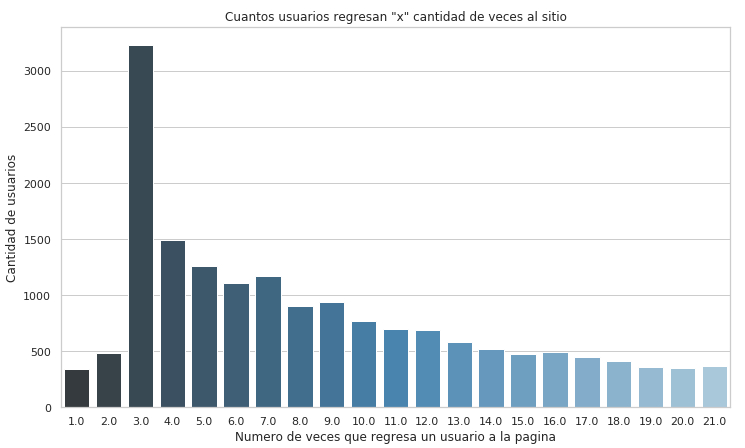
\includegraphics[width=14cm]{barrasRegresos.jpg}\\
	\textbf{Figura:}  \textit{Cantidad de usuarios por número de regresos a la página}
	\end{center}
	
	\subsection{Generic listing}
	Visitas a la página principal
	
	\subsubsection{Análisis individual de las caracterísiticas}
	Analizaremos en primer lugar cuáles son los productos que reciben mayor cantidad de visitas en la página principal.
	
	\begin{center}
    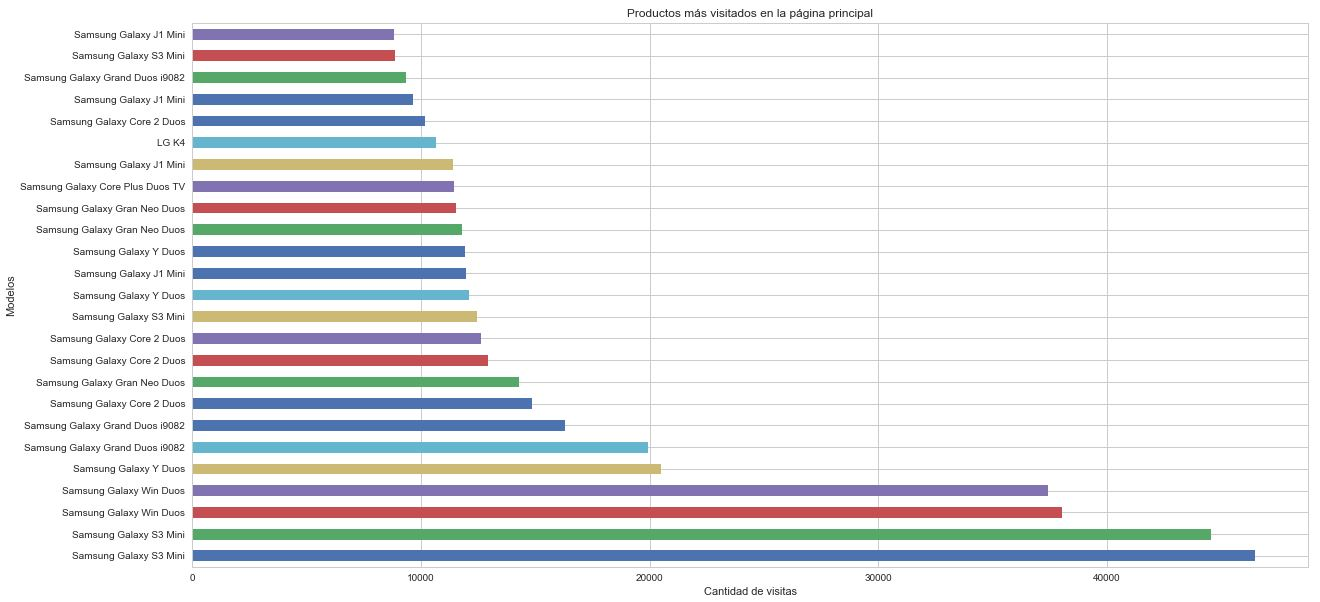
\includegraphics[width=14cm, height=9cm]{productosMasVisitadosEnLaPaginaPrincipal.jpg}\\
	\textbf{Figura:}  \textit{Cantidad de usuarios por número de regresos a la página}
	\end{center}
	
	Es evidente una clara superioridad por parte de los productos de Samsung en visitas a la página principal.
	
	\subsection{Searched product}
	Búsqueda de productos
	\subsubsection{Análisis individual de las caracterísiticas}
	Decidimos analizar qué es lo que más buscan los usuarios por palabras clave. El resultado fue el siguiente:
	
	\begin{center}
	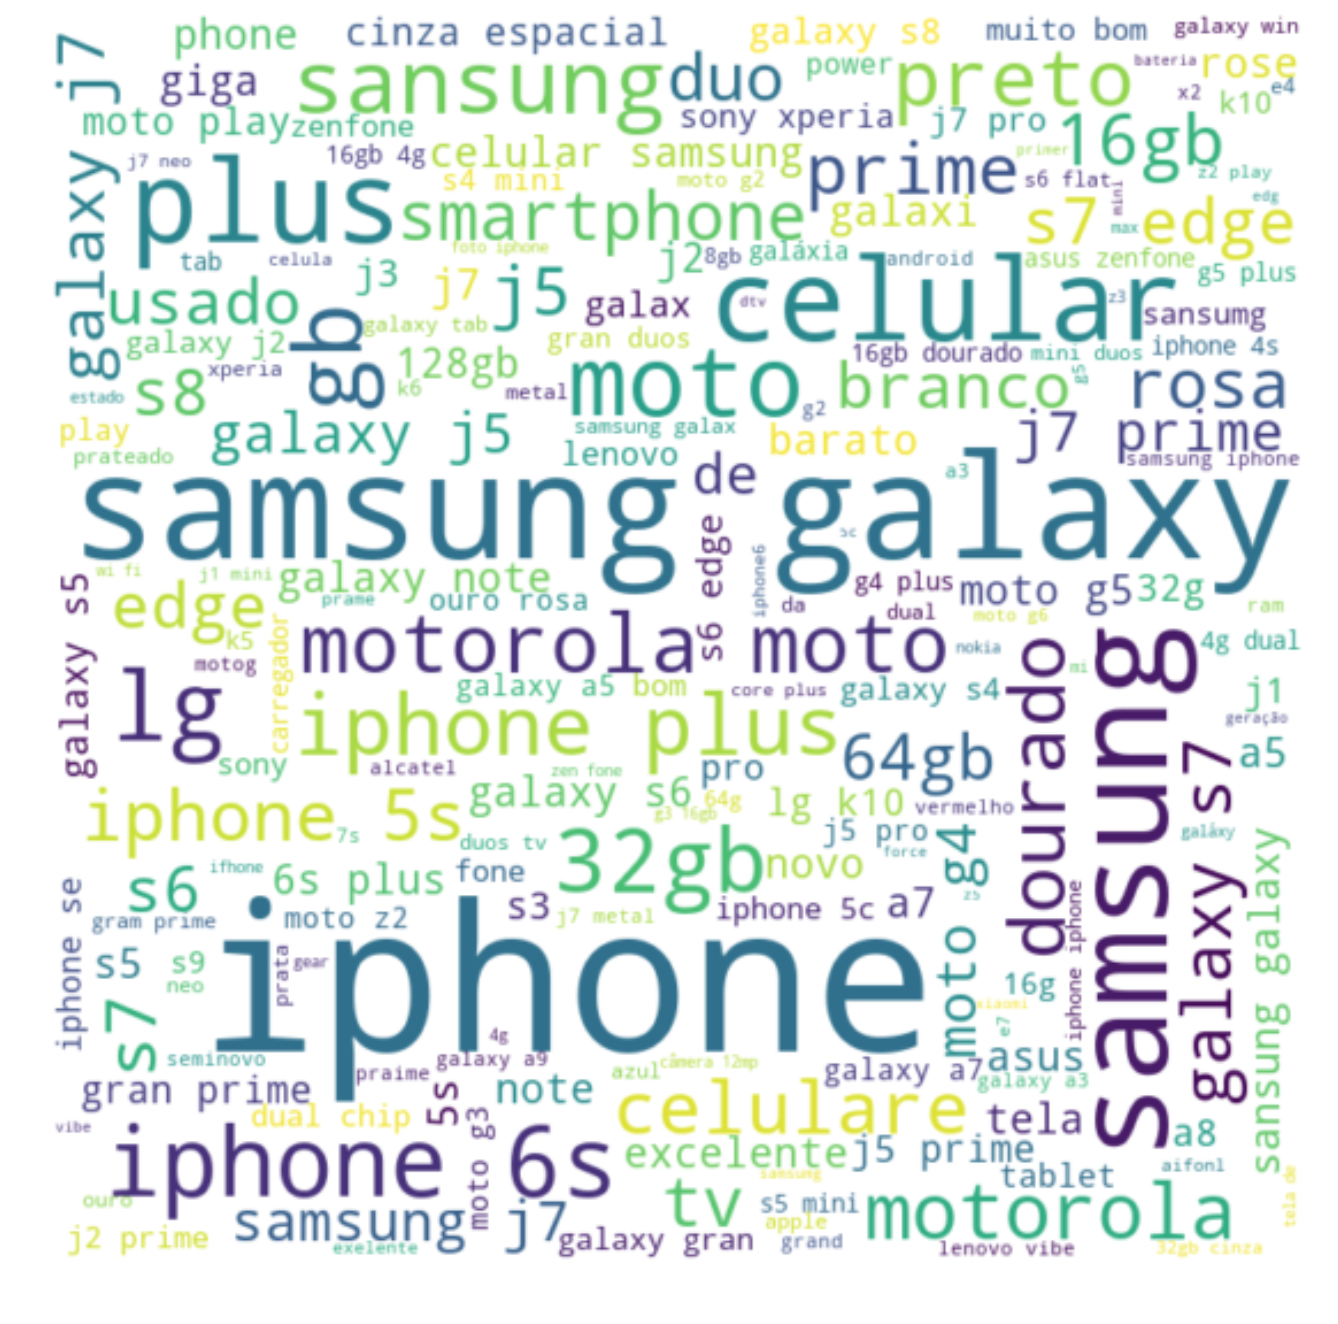
\includegraphics[width=13cm] {palabrasQueMasBuscanLosUsuarios.jpg}\\
	\textbf{Figura 23:}  \textit{Las palabras que más buscan los usuarios. }
	\end{center}
	
	Las palabras que aparecen más grande son aquellas que más se buscan.
	
	Por otro lado, analizaremos puntulamente cuáles son los productos más buscados
	\begin{center}
	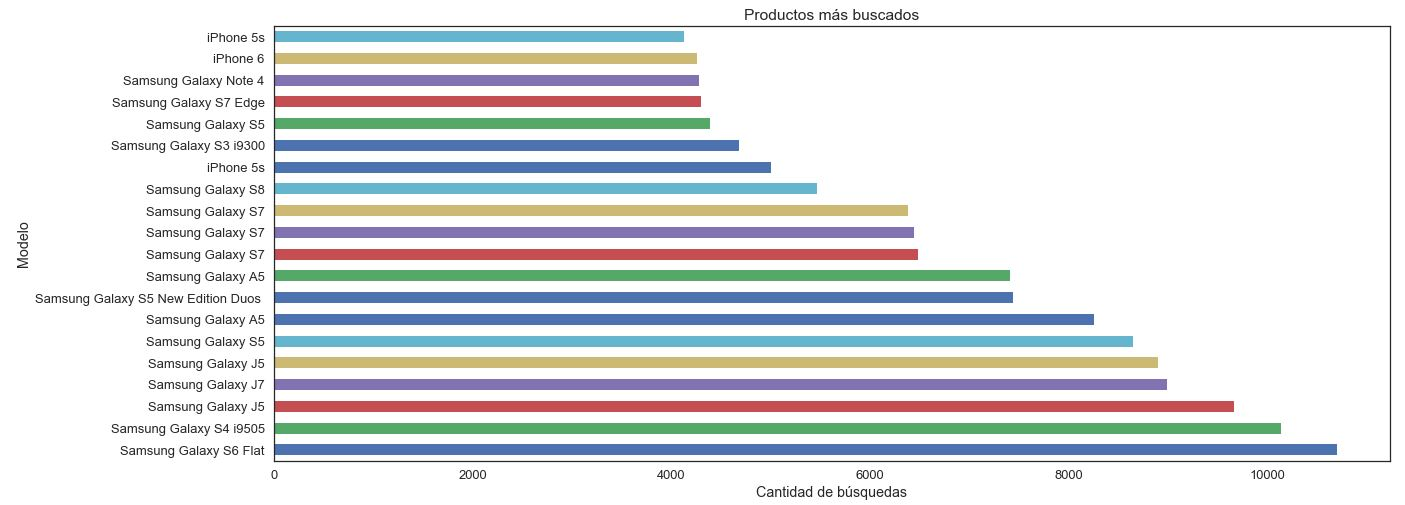
\includegraphics[width=15cm] {productosMasBuscados.jpg}\\
	\textbf{Figura 23:}  \textit{Las palabras que más buscan los usuarios. }
	\end{center} 
	
	Al igual que ocurre con las visitas hacia la página principal, podemos notar una clara superioridad por parte de Samsung a la hora de buscar modelos.
	
	\subsection{Search engine hit}
	Ingresos al sitio a través de motores de búsqueda
	\subsubsection{Análisis entre eventos}
	Analizamos la cantidad de apariciones de los buscadores. El resultado fue que el 99\% de las buquedas se realizan desde Google, entonces, el impacto de los demás buscadores es despreciable. 
	\subsubsection{Análisis temporal}
	Analizamos los ingresos a través de un motor de busqueda por día del año. El resultado fue:
	
	\begin{center}
	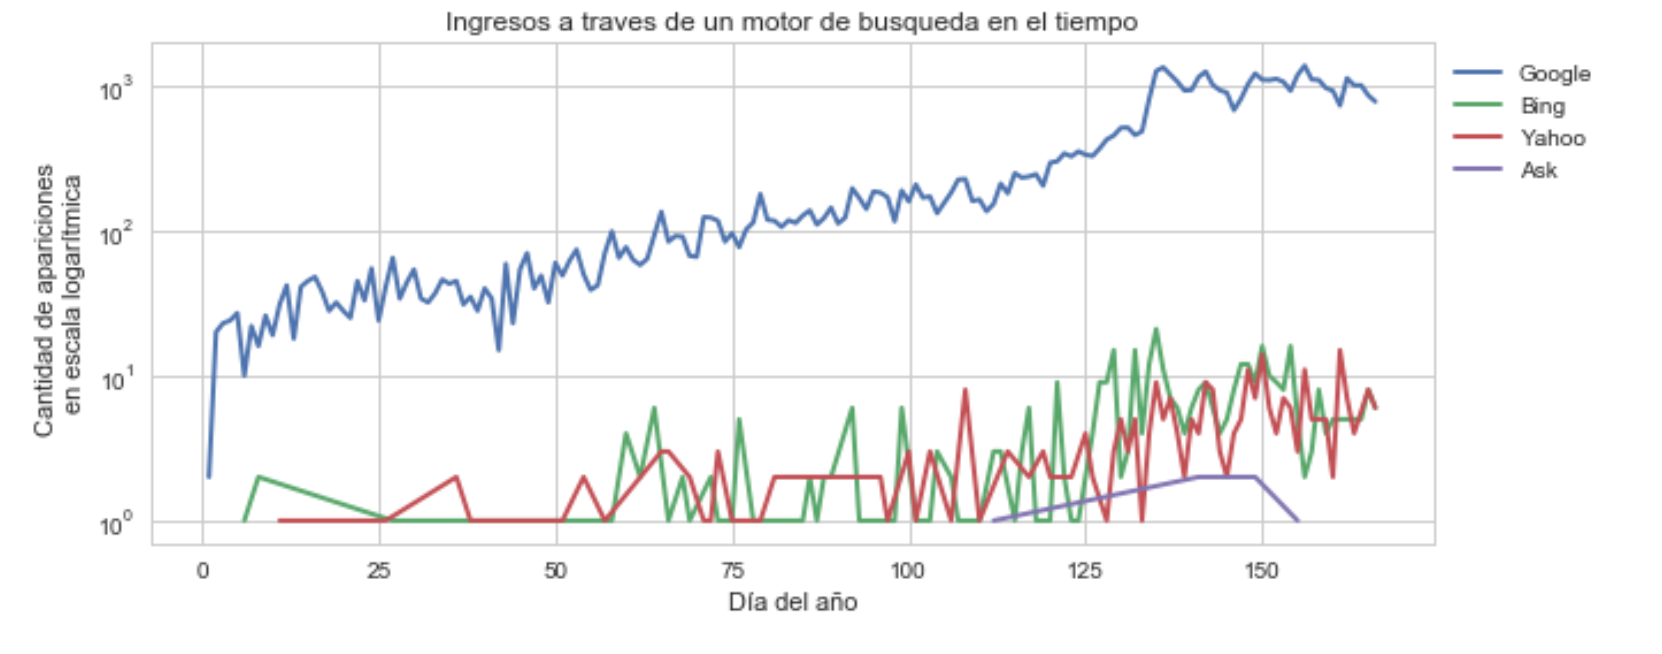
\includegraphics[width=15cm,height = 8cm]{ingresosATravesDeMotorDeBusqEnTiempo.jpg}\\
	\textbf{Figura 24:}  \textit{Ingresos a través de los motores de búsqueda a través del tiempo. }
	\end{center}
	
	Es importante mencionar que elegimos realizar el gráfico en escala logarítmica ya que la diferencia de visitas entre los buscadores es demasiado grande y no es posible apreciar la comparación a escala.\\
	Podemos observar que Google es el único buscador que posee un crecimiento estable a lo largo del tiempo, mientras que el comportamiento del resto de los buscadores es irregular.\\
	\subsection{Static page}
	Luego de analizar este evento nos dimos cuenta que no aporta información relevante en ninguno de sus campos. Las páginas estáticas poseen un volumen de visitas muy pequeño y no pudo encontrarse correlación en sus datos.
	\subsection{Conversion}
	Productos comprados por el usuario
	\subsubsection{Análisis individual entre las caracterísitcas}
	Analizamos los productos más comprados. Los 10 más comprados son:
	\begin{center}
	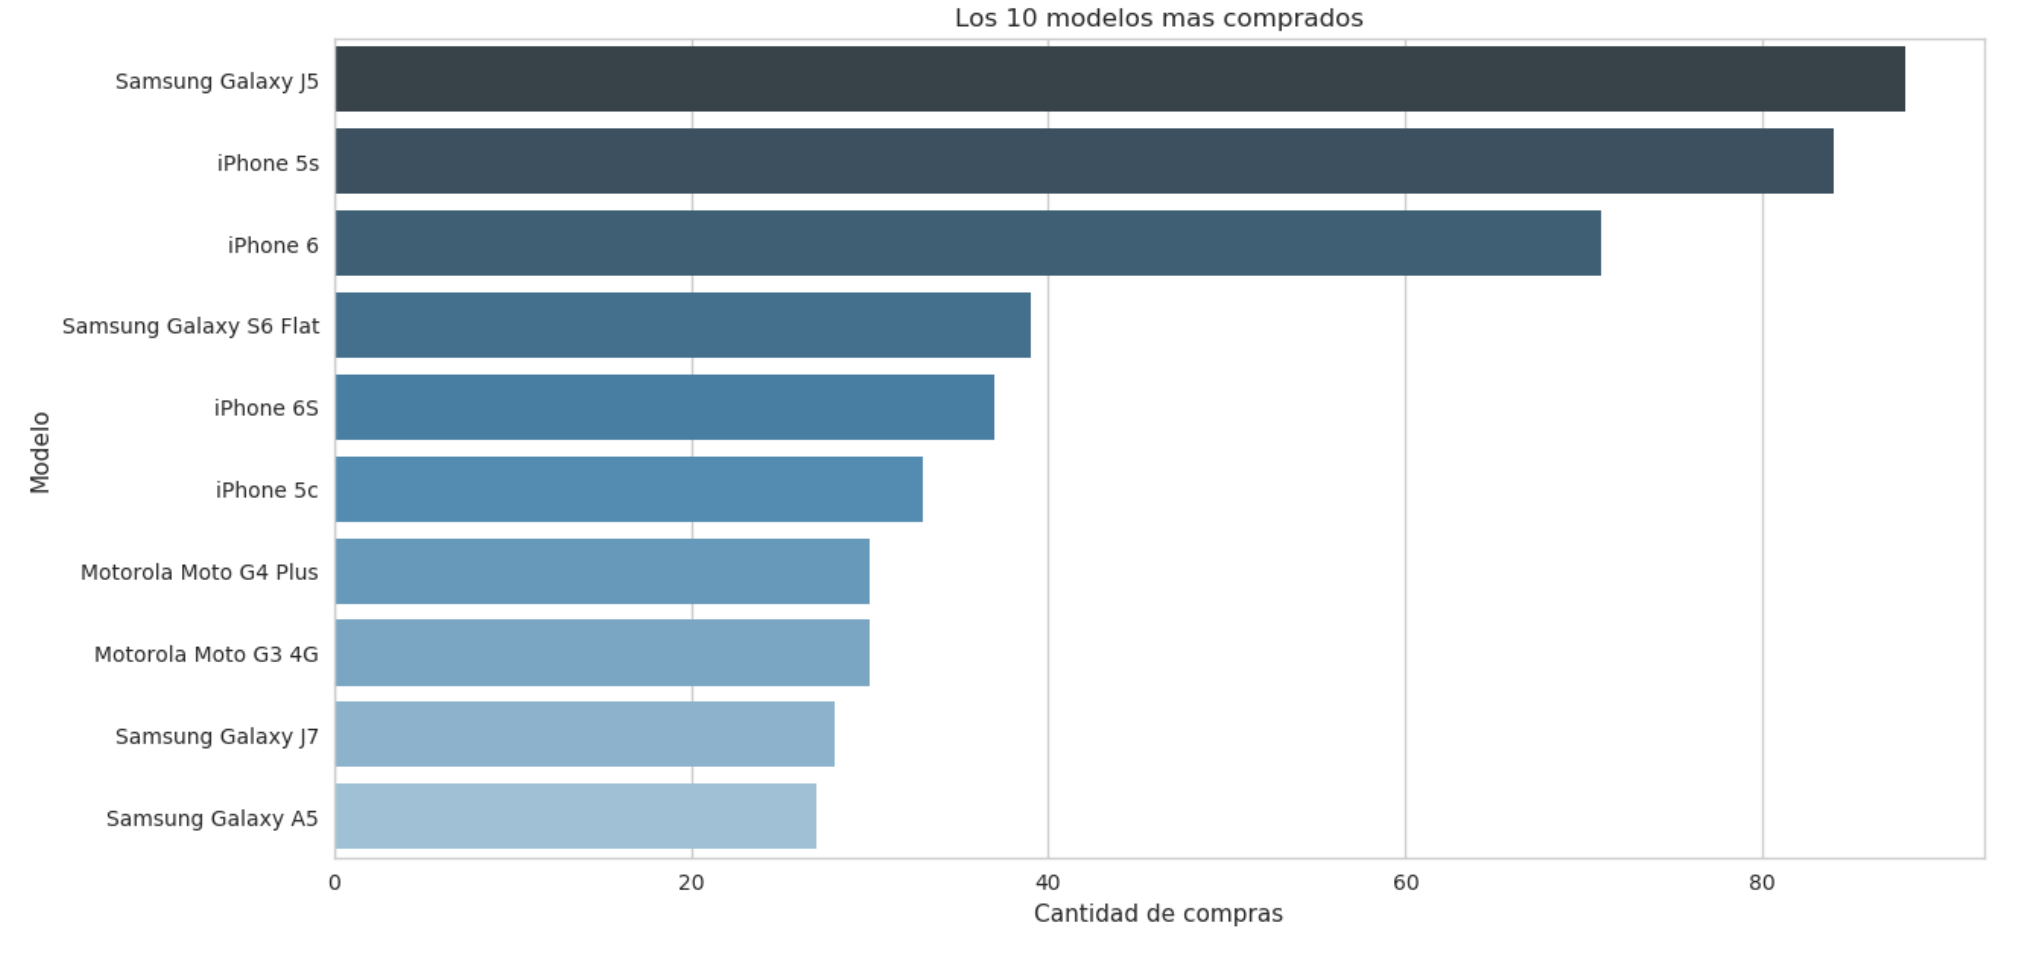
\includegraphics[width=15cm,height = 8cm]{productosMasComprados.jpg}\\
	\textbf{Figura 25:}  \textit{ Cantidad de compras según modelo. Se muestran los 10 modelos más populares. }
	\end{center}
	
	Los tres más comprados que se pueden ver son: Samsung Galaxy J5, Iphone 5S y Iphone
6. Esos son los que más se destacan por encima del resto. Luego no hay brechas muy grandes de
compras entre distintos productos. Algo que tambien es posible destacar es que, de los diez más
comprados, cuatro de ellos pertenecen a la familia de los Samnsung Galaxy, cuatro son de la marca
Apple, y dos pertenecen a la familia de los Motorola Moto G

	Analizaremos la condición de los productos comprados: 
	\begin{center}
	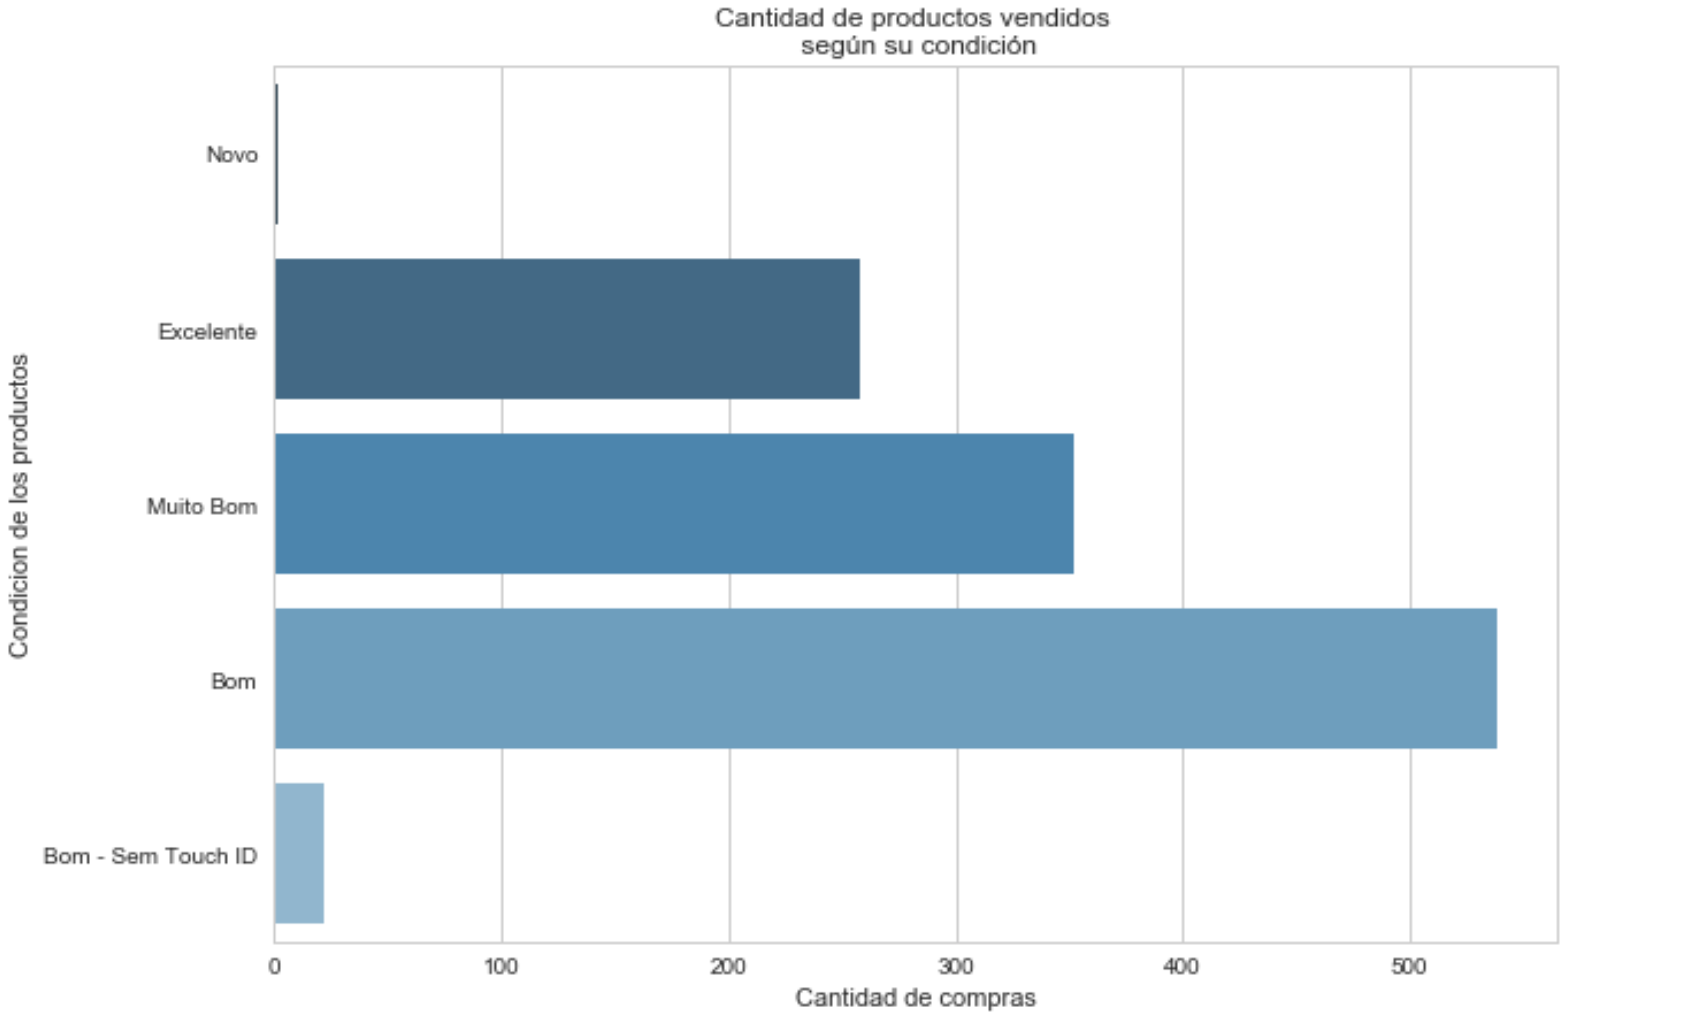
\includegraphics[width=15cm,height = 8cm]{cantidadDeProductosVendidosSegunSuCondicion.jpg}\\
	\textbf{Figura 26:}  \textit{Cantidad de productos comprados según su condición. }
	\end{center}
	
	  Aquí se puede observar que los que más compras tienen son los que tienen, relativamente, peor condición (condición: Bien). Esto puede llevar a pensar que gran parte de los usuarios al hacer una compra no priorizan la condición del producto. Aunque cabe destacar que se deberia tener en cuenta cuantos productos de cada condicion posee la pagina.
	  
	
	\section{Análisis entre eventos}
	\subsection{Visitas por campaña publicitaria VS conversiones a lo largo del tiempo}
	En esta sección analizaremos la relación entre eventos. 
	Se buscará una relación entre los \textit{clicks} de las campañas publicitarias con las visitas y las compras de los productos. 	Lo obtenido fue lo siguiente:
	\begin{center}
	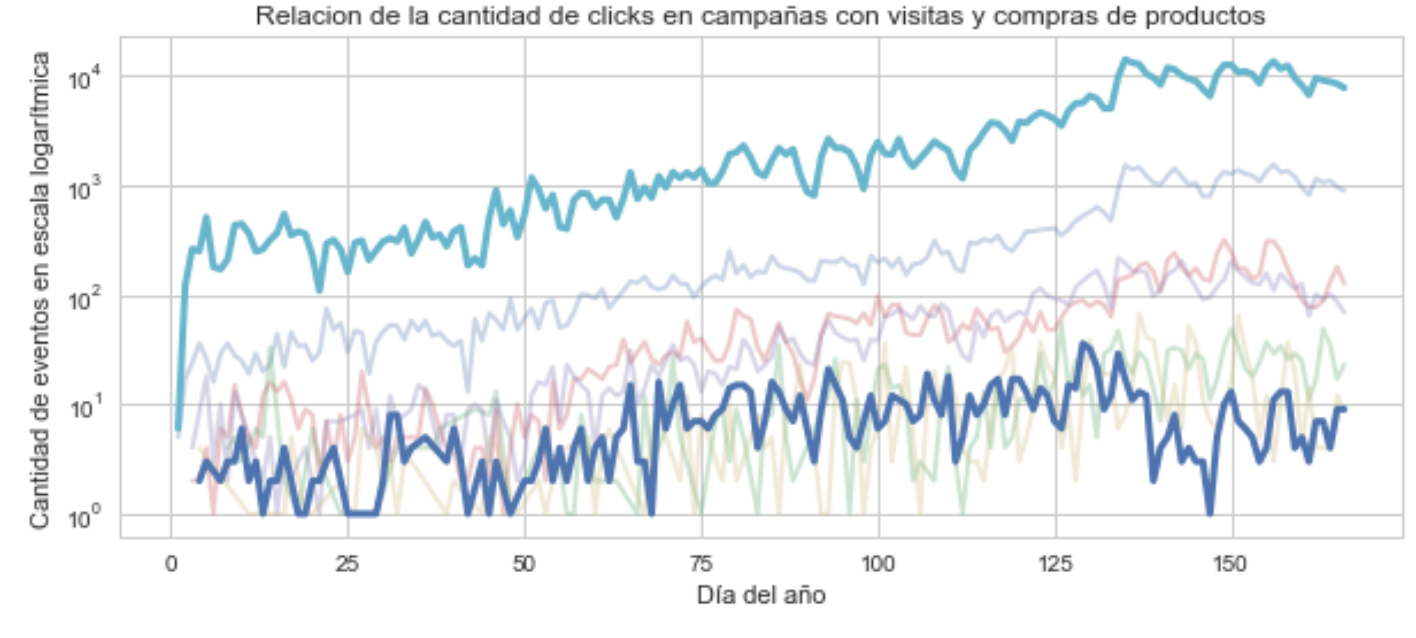
\includegraphics[width=15cm,height = 8cm] {RelacionCampaniaYConversion.jpg}\\
	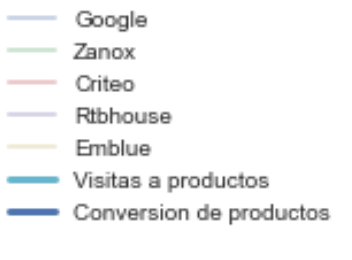
\includegraphics[width = 3cm, height = 3cm]{RelacionCampaniaYConversionCuadrito}
	\textbf{Figura 27:}  \textit{ Relación entre los clicks en las campañas publicitarias con las visitas y compras de los productos .}
	\end{center}
	Podemos ver que a medida que aumentan los clicks en las campañas publicitarias, tambien
lo hacen las visitas a productos, lo cual es lógico. Algo quizas no tan esperado es que aunque aumentan
las visitas y los clicks en las publicidades, las conversiones no parecen aumentar. En la primer mitad podemos
ver que era más baja la cantidad de conversiones, pero luego distingimos que estas se mantienen aproximadamente 
constantes a pesar del incremento en las visitas.

	\subsection{Relación entre número de compras y visitas para un mismo usuario}
  Un posible análisis para esta sección es tomar cada usuario que entró alguna vez al sitio y ver cuantas compras y cuantas visitas a productos posee.
  
  Para eso realizamos un scatter plot en donde cada punto en el plano es un cliente que posee una cantidad total de visitas al sitio (eje \textit{y}) y una cantidad total de compras (eje  \textit{x}).
  
	\begin{center}
	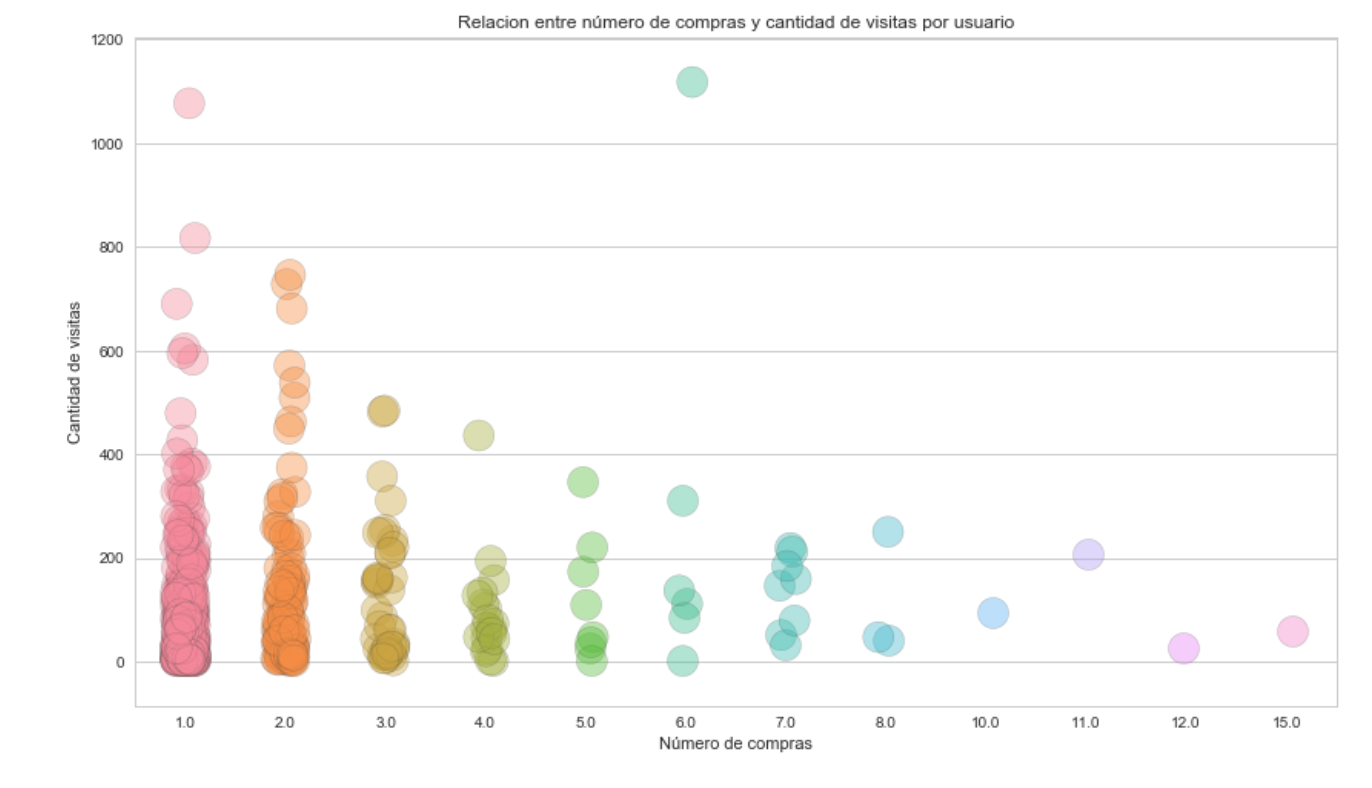
\includegraphics[width=15cm,height = 8cm] {relacionEntreComprasYCantidadDeVisitas.jpg}\\
	\textbf{Figura 28:}  \textit{ Relación entre el número de compras y cantidad de visitas por usuarios.}
	\end{center}
	
	En el gráfico claramente se puede observar que la mayoria de los usuarios hace 1 o 2 compras como mucho y visitan la pagina una cantidad relativamente baja de veces. Tambien es posible observar que, en general, los compradores que hacen más visitas son usuarios que hacen pocas compras. A mayor cantidad de compras, se ven menos cantidad de usuarios y, ademas, son usuarios que visitan pocas veces el sitio en comparación a los otros compradores.
	
	 \subsection{Análisis sobre las campañas de Marketing}
	\subsubsection{Análisis general}
	Un punto importante que podemos analizar es : ¿Qué campañas de marketing se las puede considerar más  \textit{eficientes}?
	
	Para intentar responder a esta pregunta, vimos cuantos usuarios entran por cada campaña y de éstos filtramos a los usuarios que compraron uno o más productos alguna vez. Así obtuvimos a la cantidad de compradores que ingresan al sitio por campaña.
	
	
	 \begin{center}
   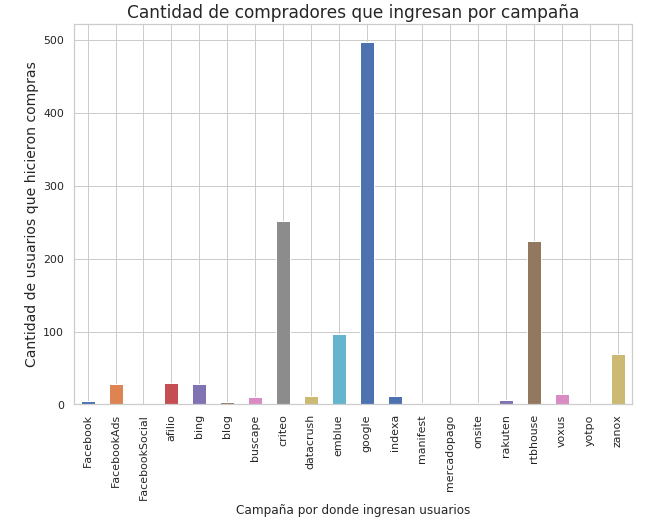
\includegraphics[width=14cm]{compradoresPorCamp.jpg}\\
	\textbf{Figura:}  \textit{Cantidad de compradores que ingresan por \textit{x} campaña de marketing}
	\end{center}
	
		 Aquí se puede ver qué cantidad de usuarios que ingresaron alguna vez al sitio por una campaña de marketing hicieron una (o más) compras. Esto no quiere decir que estos mismos usuarios entraron al sitio mediante la campaña y realizaron una compra inmediatamente. Sólo se tomaron en cuenta los que hicieron alguna compra, sin reestricciones temporales. Además, un usuario puede haber entrado al sitio por más de una campaña a lo largo del año.
	
	Como se ve en el gráfico, la gran mayoría ingresa por la campaña de Google. Los dos siguientes más destacados son Criteo y Rtbhouse.
	
	Para hacer una mejor comparación, obtuvimos la cantidad total de usuarios que ingresan por cada campaña y, con los datos del gráfico anterior, pudimos calcular qué porcentaje del total de éstos que ingresa por cada campaña son compradores.

	 \begin{center}
   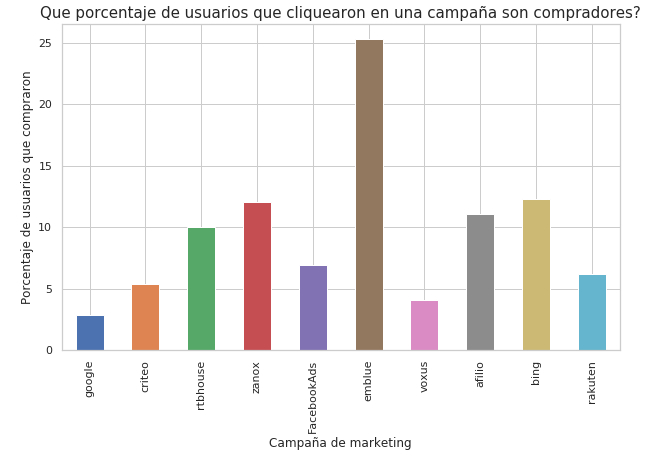
\includegraphics[width=14cm]{usuariosPorCampPorcent.jpg}\\
	\textbf{Figura:}  \textit{Porcentaje de usuarios que ingresan por cada campaña de marketing que son compradores}
	\end{center}
	
	Los datos que parecen ser más relevantes son los siguientes: \\
	
- Campaña \textit{emblue} con un 25.26 porciento de compradores (97 de 348)

- Campaña \textit{bing} con un 12.28 porciento de compradores (28 de 228)

- Campaña \textit{zanox} con un 12.0 porciento de compradores (69 de 572)

- Campaña \textit{rtbhouse} con un 9.99 porciento de compradores (224 de 2241)

- Campaña \textit{google} con un 2.86 porciento de compradores (497 de 17372)\\


Cabe destacar que, a pesar de que la campaña de marketing de \textit{Google} en este gráfico es la de menos porcentaje de compradores, es la campaña en la cual se registró la mayor cantidad de compradores (497) y mayor trafico de usuarios (17372 usuarios distintos).\\

Algo a resaltar es que la campaña de marketing de \textit{emblue} es la que más se destaca del resto en el último gráfico. Es la sexta campaña con más usuarios que cliquearon (348) y la que mejor porcentaje de compradores tiene (25.26\%. Es decir: 97 de 348), siendo la cuarta con mas cantidad de compradores.


  \subsubsection{Modelos más comprados por usuarios que cliquearon una determinada campaña}

	La pregunta que nos motivó en el análisis de esta sección fue la siguiente: ¿Se comportan de forma distinta los usuarios en cuanto a las compras de los diferentes modelos dependiendo de la campaña por la cual ingresan?

	Para eso, vimos cuantos usuarios entran por cada campaña. De estos filtramos a los usuarios que compraron uno o más productos alguna vez y seleccionamos esos productos, obteniendo la cantidad de usuarios que compraron cada producto.
	
		
	\begin{center}
   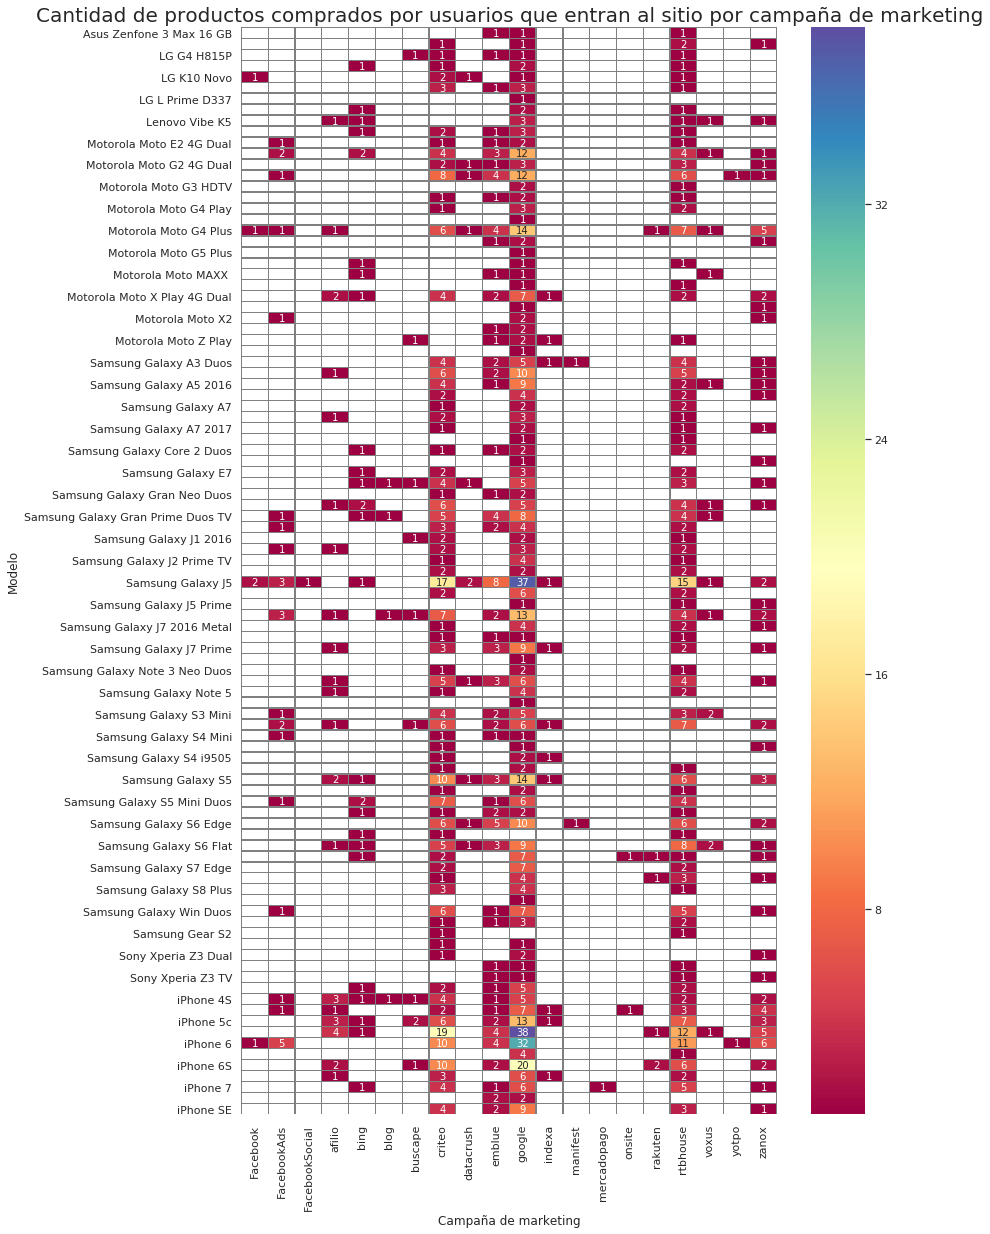
\includegraphics[width=14cm, height=20cm]{modelosCamp.png}\\
	\textbf{Figura:}  \textit{Cantidad de modelos comprados por \textit{x} campaña de marketing que son compradores.}
	\end{center}
	
	Hacemos una reestricción y miramos las tres campañas de marketing más relevantes:
	
  \begin{center}
   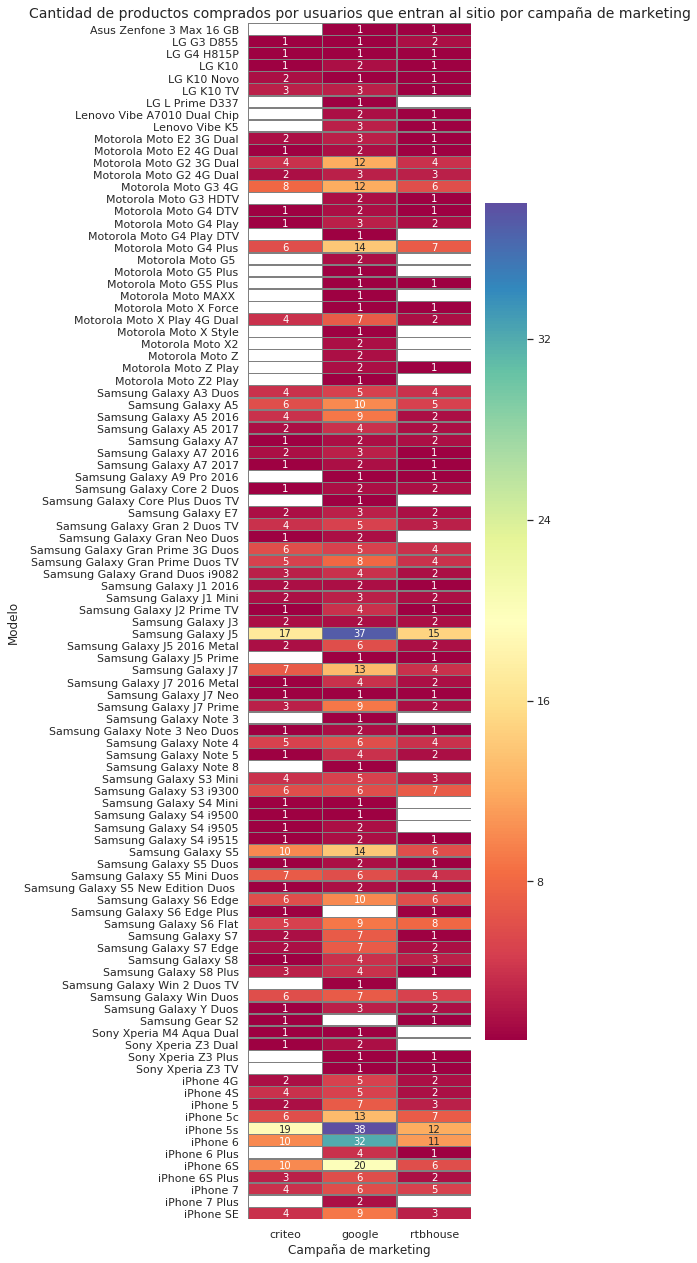
\includegraphics[width=14cm, height=21.5cm]{modelosCamp2.png}\\
	\textbf{Figura:}  \textit{Cantidad de modelos comprados por \textit{x} campaña de marketing que son compradores}
	\end{center}
	
	Podemos ver solo los productos que estan en todas las filas:

  \begin{center}
   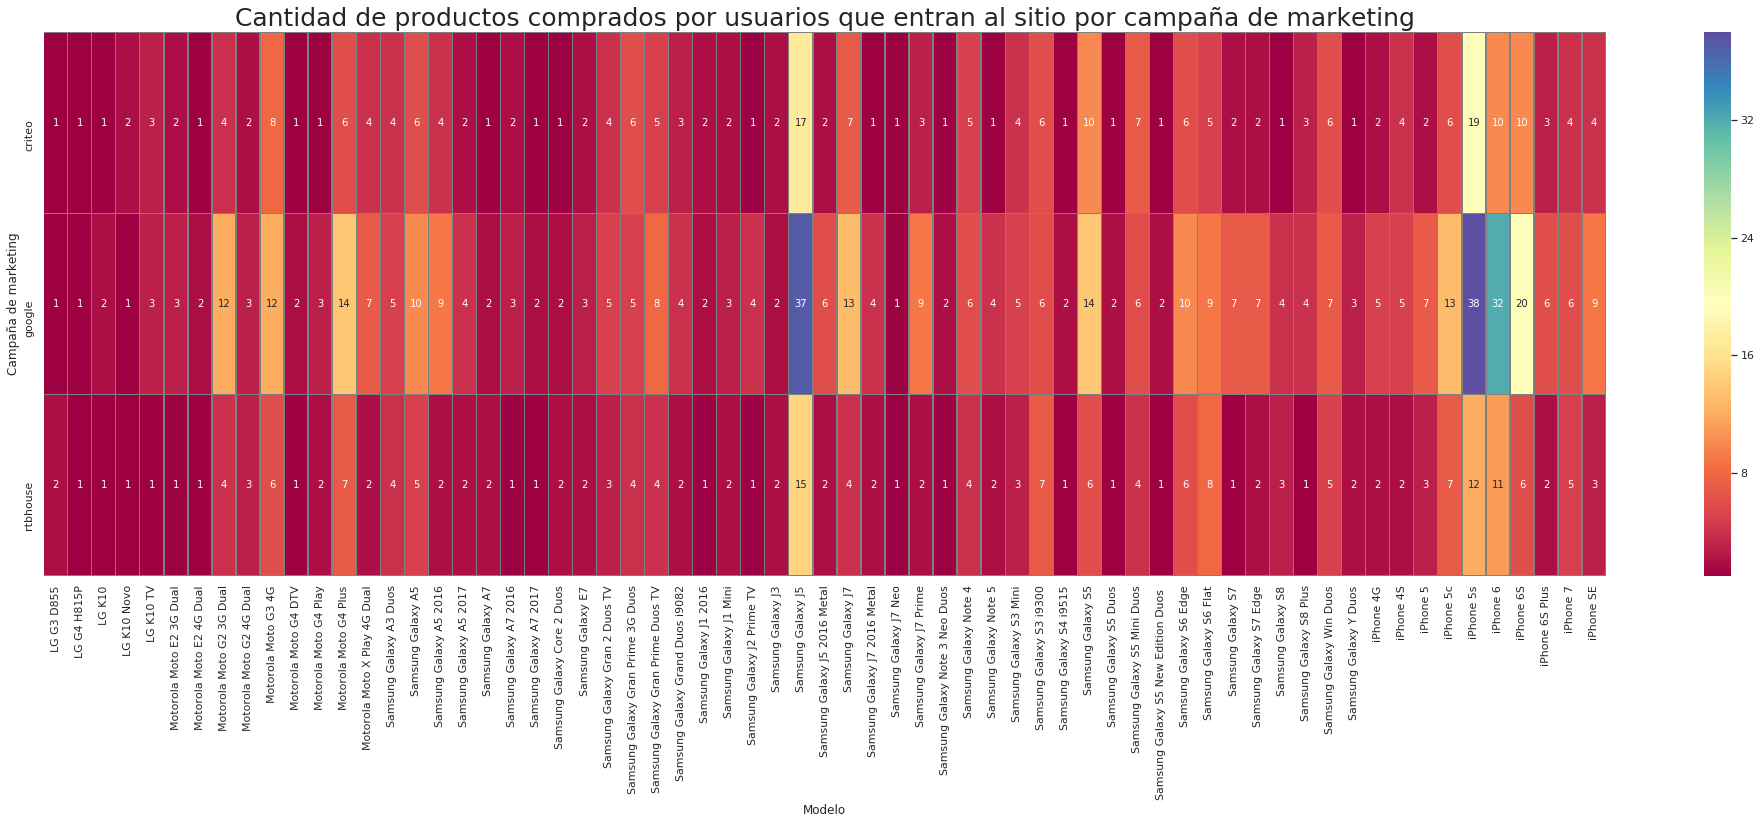
\includegraphics[width=16cm, height=7cm]{modelosCamp3.png}\\
	\textbf{Figura:}  \textit{Cantidad de modelos comprados por \textit{x} campaña de marketing que son compradores}
	\end{center}	
	
	
Observando estos graficos pudimos concluir que no es posible destacar un comportamiento de usuarios haciendo una division por campaña de marketing. Más allá de la diferencia de cantidades de compradores entre campañas, la tendencia a comprar determinados productos, en general, es la misma. Por esto no se puede decir que los usuarios que entran al sitio por una campaña especifica tienen distinto comportamiento a los usuarios que entran mediante otras campañas (respecto a las compras de los diferentes productos).

Esto puede relacionarse con el grafico de tiempo que muestra las compras y las entradas por distintas campañas.
	
	
	\subsection{Análisis de dispositivos}
	El 98\% de los usuarios que han ingresado al sitio lo han hecho con un mismo tipo de dispositivo. Siendo que el 2\% ha ingresado al sitio con varios tipos de dispositivo (Computadora, Smartphone, tablet, etc). Despreciando este 2\%, podemos decir que los usuarios que ingresan al sitio lo hacen utilizando siempre el mismo tipo de dispositivo. \\
	
	Partiendo de esta premisa, podemos realizar los siguientes análisis.
	
	\subsubsection{Análisis de sistemas operativos}
	
	  \begin{center}
	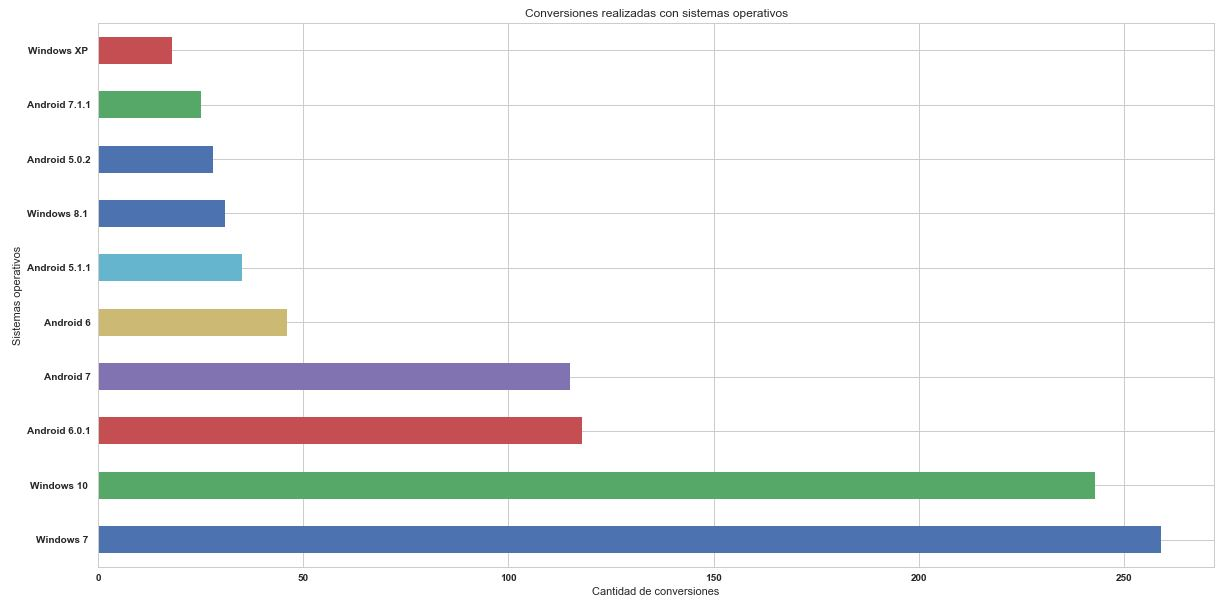
\includegraphics[width=16cm]{conversionesRealizadasPorSistemaOperativo.jpg}\\
	\textbf{Figura:}  \textit{Cantidad de modelos comprados por \textit{x} campaña de marketing que son compradores}
	\end{center}
	
	
	Podemos observar que la mayoría de las conversiones se realizan desde sistemas operativos Windows 7 y Windows 10 (Computadoras).
	
	\begin{center}
	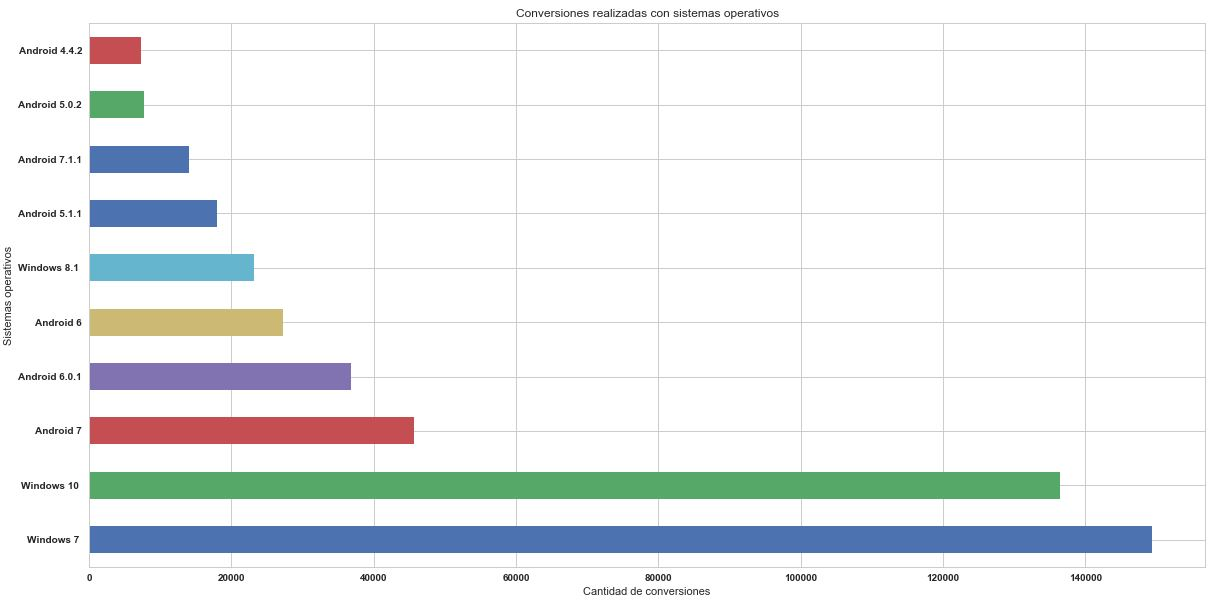
\includegraphics[width=16cm]{visitasRealizadasPorSistemaOperativo.jpg}\\
	\textbf{Figura:}  \textit{Cantidad de modelos comprados por \textit{x} campaña de marketing que son compradores}
	\end{center}
	
	\textbf{Observación} Si bien el sistema operativo más usando para visualizar productos es Windows, la mayor cantidad de visitas en total se producen a través de Smartphones, se supone que esto se dará a causa de la gran cantidad de sistemas operativos que hay en mobile, lo que provoca que la categoría Smartphones se disperse.
	
	\subsubsection{Análisis de resoluciones}

	\begin{center}
	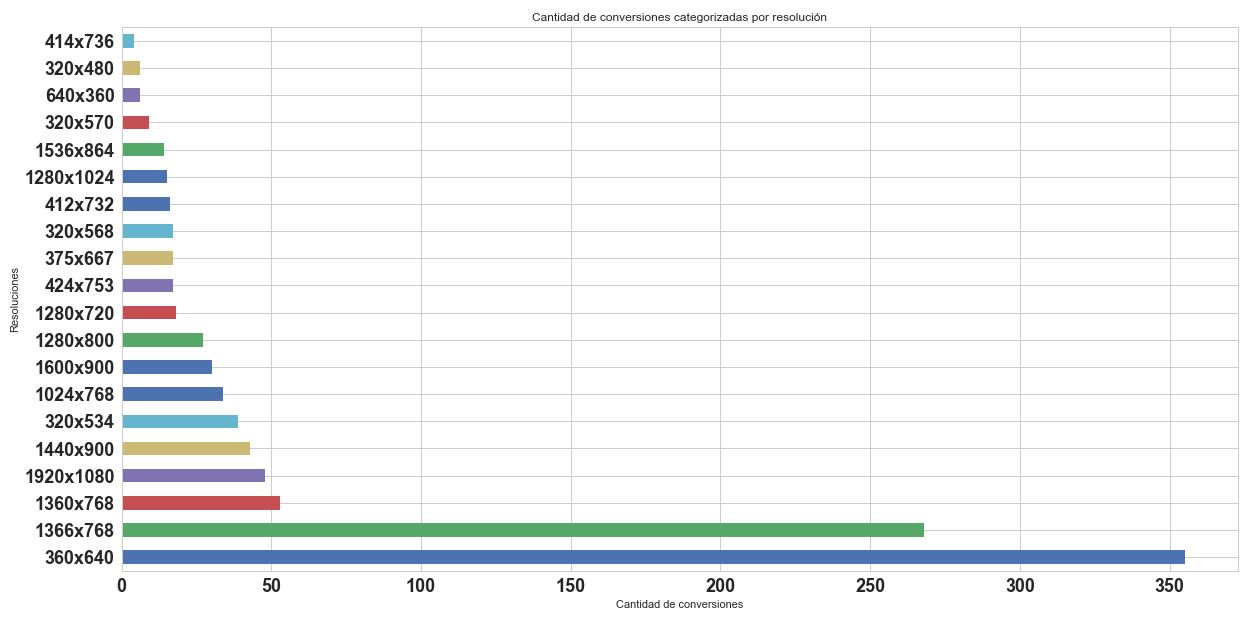
\includegraphics[width=16cm]{conversionesRealizadasPorResolucion.jpg}\\
	\textbf{Figura:}  \textit{Cantidad de modelos comprados por \textit{x} campaña de marketing que son compradores}
	\end{center}
	
	Podemos notar que la mayor cantidad de conversiones se realizan desde dispositivos con resolución de computadora. Sin embargo hay un dato que genera ruido.
	
	\subsection{Productos más populares por ciudad de Brasil}
	
	\begin{center}
	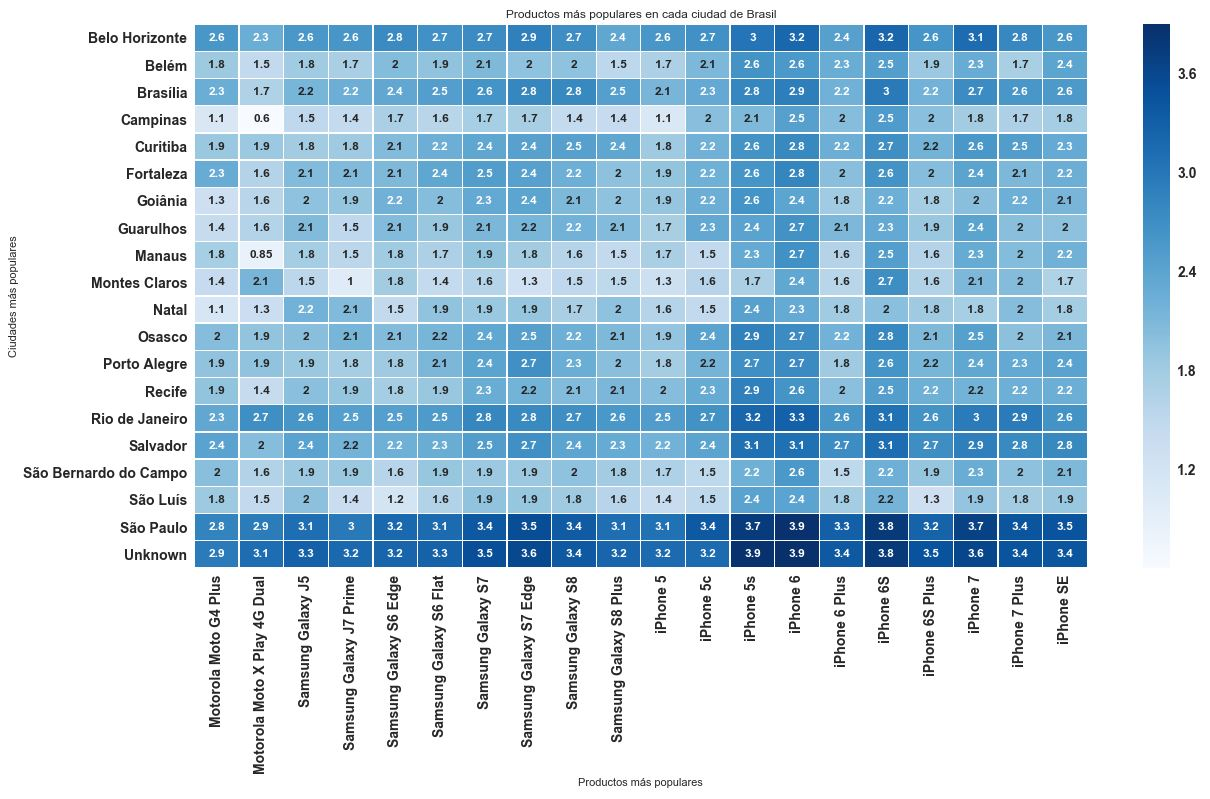
\includegraphics[width=16cm]{productosMasVisitadosPorCiudadDeBrasil.jpg}\\
	\textbf{Figura:}  \textit{Cantidad de modelos comprados por \textit{x} campaña de marketing que son compradores}
	\end{center}
	
	Podemos notar que Sao Paulo y Unknown son las zonas que concentran la mayor cantidad de actividad.
		
	\subsection{Conversiones en base a checkouts}
	
	\begin{center}
	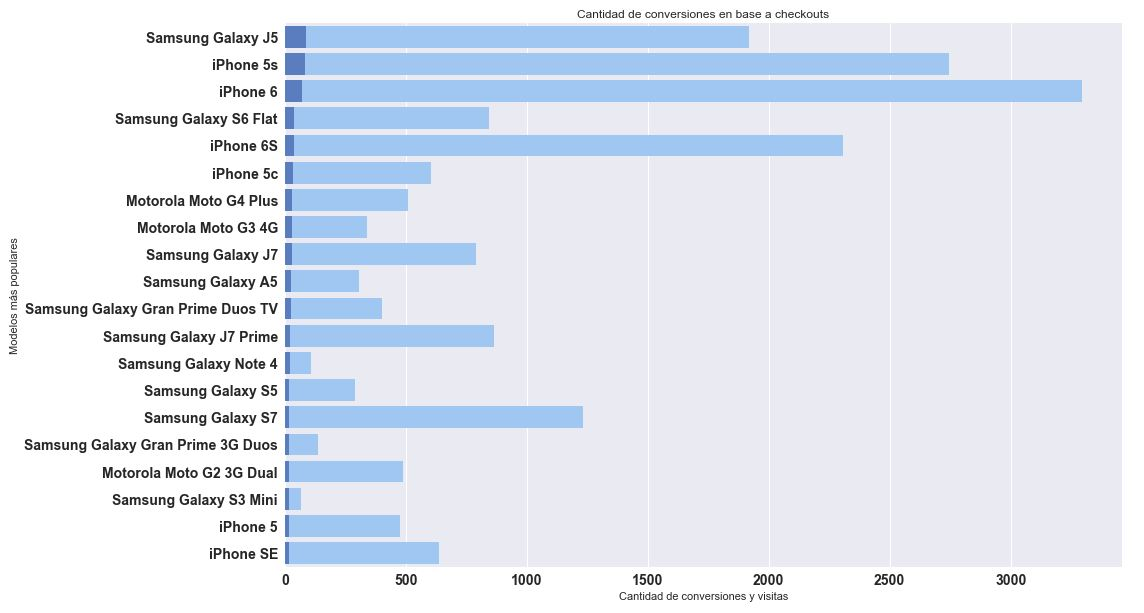
\includegraphics[width=16cm]{conversionesEnBaseACheckouts.jpg}\\
	\textbf{Figura:}  \textit{Cantidad de modelos comprados por \textit{x} campaña de marketing que son compradores}
	\end{center}
		
\end{document}